\documentclass[]{scrartcl}

\usepackage{amsmath}
\usepackage{amssymb}
\usepackage[utf8]{inputenc}
\usepackage[T1]{fontenc}
\usepackage{lmodern}
\usepackage{ngerman}
\usepackage{geometry}
\usepackage{graphicx}
\usepackage{wrapfig}
\usepackage{caption}
\usepackage{wasysym}
\usepackage[separate-uncertainty = true,multi-part-units=single]{siunitx}
\usepackage{picinpar}
\usepackage{tikz}
\usepackage{float}
\usepackage{booktabs}


\renewcommand{\figurename}{Abb.}
\usepackage[
	colorlinks=true,
	urlcolor=blue,
	linkcolor=black
]{hyperref}

%Hier Titel und so
\newcommand{\versuchnummer}{V51} 
\newcommand{\versuchname}{Schaltungen mit Operationsverstärkern} 
\newcommand{\versuchdatum}{28.11.16} 

\hyphenation{Ausgangs-spannung Eingangs-widerstand Linear-verstärker}

\let\oldsection\section
\renewcommand\section{\clearpage\oldsection}

\title{Versuch \versuchnummer\\ \versuchname}
\subtitle{Physikalisches Fortgeschrittenenpraktikum}
\author{Robert Rauter und Björn Lindhauer}
\date{\versuchdatum} 
\begin{document}
\begin{titlepage}
{\large \versuchdatum}
\vspace{7cm}
\begin{center}
\textbf{\huge Versuch \versuchnummer:}\\
\vspace{0.5cm}
\textbf{\huge \versuchname}\\
\vspace{0.2cm}
\textbf{ Physikalisches Fortgeschrittenenpraktikum}\\
\vspace{0.2cm}
\textbf{Korrigierte Version des Protokolls}\\
\vspace{9cm}

{\Large Robert Rauter \ \ \hspace{1.5cm} und \hspace{1.5cm} Björn Lindhauer}\\
{ \url{robert.rauter@tu-dortmund.de} \ \ \hspace{2cm} \url{bjoern.lindhauer@tu-dortmund.de}}
\end{center}
\end{titlepage}

\tableofcontents

\section{Einleitung}
Mithilfe von Operationsverstärkern können Signale verstärkt werden. Werden Operationsverstärker sinnvoll mit Kondensatoren und Widerständen kombiniert, so ist die Erzeugung von besonderen Signalen, wie zum Beispiel einem Dreiecksignal , möglich. \\
In diesem Versuch soll untersucht werden, wie mit verschiedenen Schaltungen verschiedene Verstärkungsgrade realisiert werden können. Au"serdem sollen komplexere Schaltungen zur Erzeugung eines Dreieckssignals und einer exponentiell abfallenden Schwingung realisiert werden.

\section{Theoretische Grundlagen}
\subsection{Ideale Operationsverstärker}
Ein Operationsverstärker wird durch das Schaltsymbol in Abbildung  \ref{fig:schaltsymbol_operationsverstaerker} repräsentiert und ist ein elektronisches Bauteil, dessen Ausgangsspannung
\begin{align}
 U_{\text{A}}=V\cdot \left( U_{\text{P}}-U_{\text{N}} \right)
\end{align}
ist, welche somit proportional zur Differenz an den beiden Eingängen ist.
Deswegen wir er auch als gleichstromgekoppelter Differenzverstärker bezeichnet.

\begin{figure}[H]
\centering
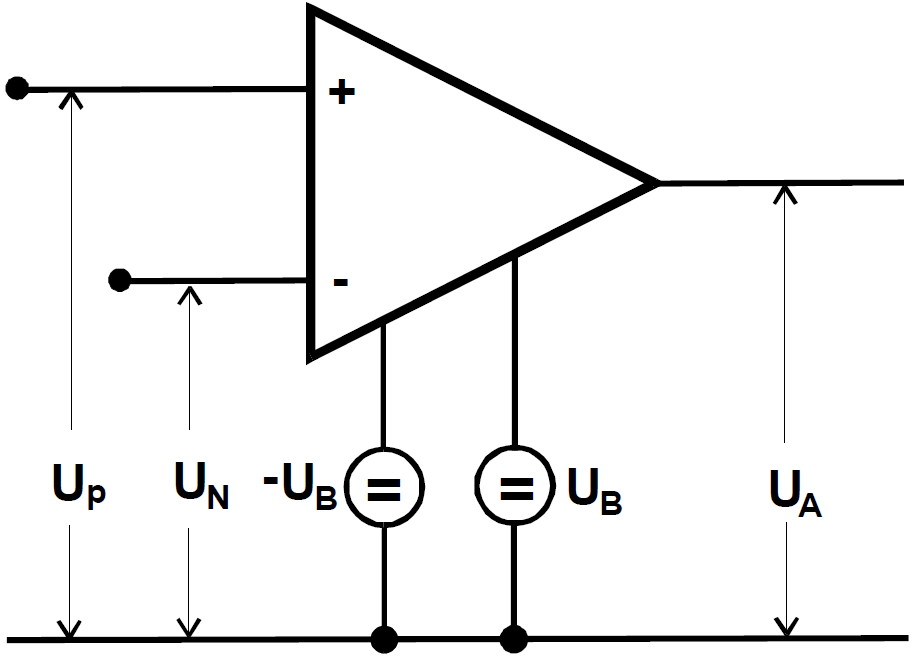
\includegraphics[width=7cm]{images/schaltsymbol_operationsverstaerker.png}
\caption{Schaltsymbol eines Operationsverstärkers. Die Betriebsspannung $\pm U_{\text{B}}$ wird jedoch häufig nicht mit eingezeichnet. [1]}
\label{fig:schaltsymbol_operationsverstaerker}
\end{figure}

Die Betriebsspannung $\pm U_{\text{B}}$ limitiert das Ausgangssignal $U_{\text{A}}$ auf dem Bereich
\begin{align}
 -U_{\text{B}} < U_{\text{A}} < U_{\text{B}}
\end{align}
und sorgt für eine Sättigung bei $\left| U_{\text{A}} \right| > U_{\text{B}}$. Der Verlauf der Kurve ist in Abbildung \ref{fig:kennlinie_operationsverstaerker} schematisch dargestellt. 

Es wird der Eingang mit der Spannung $U_{\text{P}}$ als nicht-invertierter Eingang (+) bezeichnet, da die Ausgangs\-spannung $U_{\text{A}}$ in Phase mit der Spannung $U_{\text{P}}$ ist.
Die Ausgangsspannung ist jedoch gegenphasig zur Spannung $U_{\text{N}}$, weshalb deren Eingang als invertierter Eingang (-) bezeichnet wird.

Bei einem idealen Operationsverstärker ist die Leerlaufverstärkung $V$, sowie der Eingangswiderstand $r_{e}$ unendlich groß und der Ausgangswirderstand $r_a$ verschwindet.
Dies ist beim realen Operationsverstärker jedoch nicht der Fall, sodass es sinnvoll ist, weitere Größen zu definieren.

\begin{figure}[H]
\centering
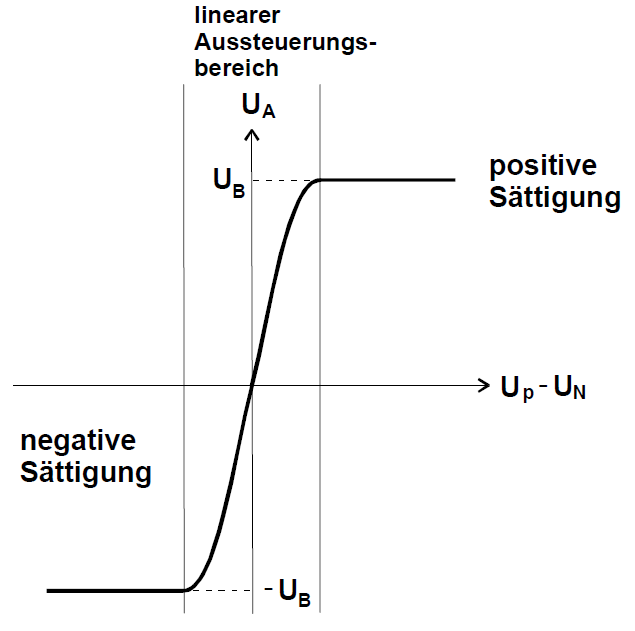
\includegraphics[width=7cm]{images/kennlinie_operationsverstaerker.png}
\caption{Kennlinie eines Operationsverstärkers. Die Steigung der Geraden zwischen den Sättigungen ist in Realität wesentlich steiler. [1]}
\label{fig:kennlinie_operationsverstaerker}
\end{figure}

\subsection{Reale Operationsverstärker}
Die Ausgangsspannung ist von Null verschieden, wenn an den beiden Eingängen die gleiche Spannung $U_{gl}$ anliegt. Deshalb wird die Gleichtaktverstärkung
\begin{align}
 V_{gl}:=\frac{\Delta U_{A}}{\Delta U_{gl}}
\end{align}
definiert. 
Aus den endlichen Eingangswiderständen folgen Eingangsruheströme $I_{P}$ und $I_{N}$, die zur Definition des Eingangsruhestroms
\begin{align}
 I_{B}:=\frac{1}{2} \cdot \left(I_{P}+I_{N}\right)
\end{align}
und des Offsetstroms
\begin{align}
 I_{0}:= \left. I_{P}-I_{N}\right|_{U_{P}=U_{N}=0} 
\end{align}
führen.
Der Differenzwiderstand wird als
\begin{align}
 r_{D}:=\left\lbrace 
\begin{array}{ll}
\frac{\Delta U_{P}}{\Delta I_{P}} & \text{, }U_{N}=0 \vspace{0.2cm}\\
\frac{\Delta U_{N}}{\Delta I_{N}} & \text{, }U_{P}=0
\end{array}
\right\rbrace 
\end{align}
definiert und der Gleichtakteingangswiderstand als
\begin{align}
 r_{gl}:=\frac{\Delta U_{gl}}{\Delta I_{gl}}
\end{align}
mit $I_{gl}=I_N+I_P$.
Da die Ausgangsspannung $U_{a}$ bei realen Operationsverstärkern ungleich null ist, wird die Offsetspannung
\begin{align}
 U_0:=\left. U_{P}-U_{N} \right|_{U_{a}=0}
\end{align}
definiert.

Diese ist häufig eine Funktion der Temperatur, Zeit und Betriebsspannung. Die totale Ableitung von $U_{0}$ wird Offsetspannungsdrift genannt.
Reale Operationsverstärker kommen idealen Operationsverstärkern sehr nahe, sodass die eingeführten Größen als Störparameter angesehen werden können und somit zu Korrekturen führen.

\subsection{Schaltungen mit Operationsverstärker}
In diesen Abschnitten sollen einige gängige Schaltungen mit Operationsverstärkern vorgestellt werden und ein paar grundsätzliche Eigenschaften der Schaltungen diskutiert werden.
\subsubsection{Linearverstärker}
Da ein Operationsverstärker bereits eine hohe Leerlaufverstärkung besitzt, ist der Ansteuerungsbereich gering und schon kleine Eingangsspannungen führen zu einer Sättigung.
\begin{figure}[H]
\centering
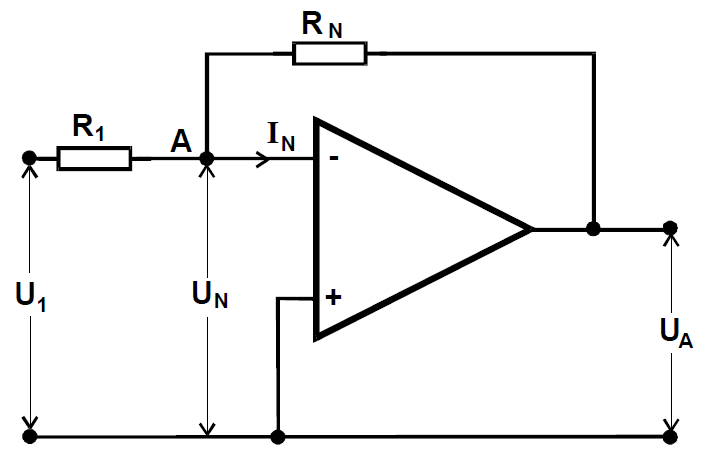
\includegraphics[width=9cm]{images/schaltplan_linearverstaerker.png}
\caption{Schaltplan eines gegengekoppelten invertierten Linearverstärkers. [1]}
\label{fig:schaltplan_linearverstaerker}
\end{figure}
Um dies zu unterbinden und höhere Eingangsspannungen zu verwirklichen, muss ein Gegenkopplungszweig, wie in Abbildung \ref{fig:schaltplan_linearverstaerker} integriert werden.

Es wird im Gegenkopplungszweig ein durch das Widerstandsverhältnis der eingebauten Widerstände bestimmter Anteil der Ausgangsspannung zurück auf den invertierten Eingang gegeben. Somit führt eine Zunahme der Ausgangsspannung zu einer Abnahme der Eingangsspannung.
Dies führt zwar zu einer Ausweitung des Ansteuerungsbereich, verringert jedoch die Gesamtverstärkung.
Die Verstärkung $V'$ ist beim idealen Operationsverstärker nur vom Verhältnis der Widerstände
\begin{align}
V'=-\frac{R_{\text{N}}}{R_{1}}
\label{eq:verstaerkung_ideal}
\end{align}
abhängig.
Die Leerlaufspannung führt zu der Korrektur Verstärkung
\begin{align}
\frac{1}{V'}\approx \frac{1}{V} + \frac{R_{1}}{R_{\text{N}}}
\label{eq:leerlaufkorrektur}
\end{align}
für große Leerlaufspannungen $V \gg 1$. Die Gleichung \ref{eq:verstaerkung_ideal} ist folglich für $\frac{R_{\text{N}}}{R_{1}} \ll V$ korrekt.
Wird eine solche starke Gegenkopplung verwirklicht, so haben thermische Fluktuationen der Leerlaufspannung nur einen kleinen Effekt auf die Schaltung, was die Stabilität der Schaltung verbessert.
Es werden durch die Gegenkopplung auch weitere Parameter positiv beeinflusst. So nimmt beispielsweise der endliche Ausgangswiderstand um den Faktor
\begin{align}
g:=\frac{V}{V'}
\end{align}
ab. Auch Schwankungen der Leerlaufverstärkung werden um den Faktor $g$ vermindert:
\begin{align}
\frac{\Delta V'}{V'}=g^{-1}\frac{\Delta V}{V}
\end{align}
Außerdem kann eine größere Frequenzbrandbreite unverzerrt übertragen werden, da diese auch um den Faktor $g$ erhöht wird. In Abbildung \ref{fig:frequenzgang_operationsverstaerker} wird der Unterschied der Brandbreiten im Frequenzgang des Linearverstärkers dargestellt.
\begin{figure}[H]
\centering
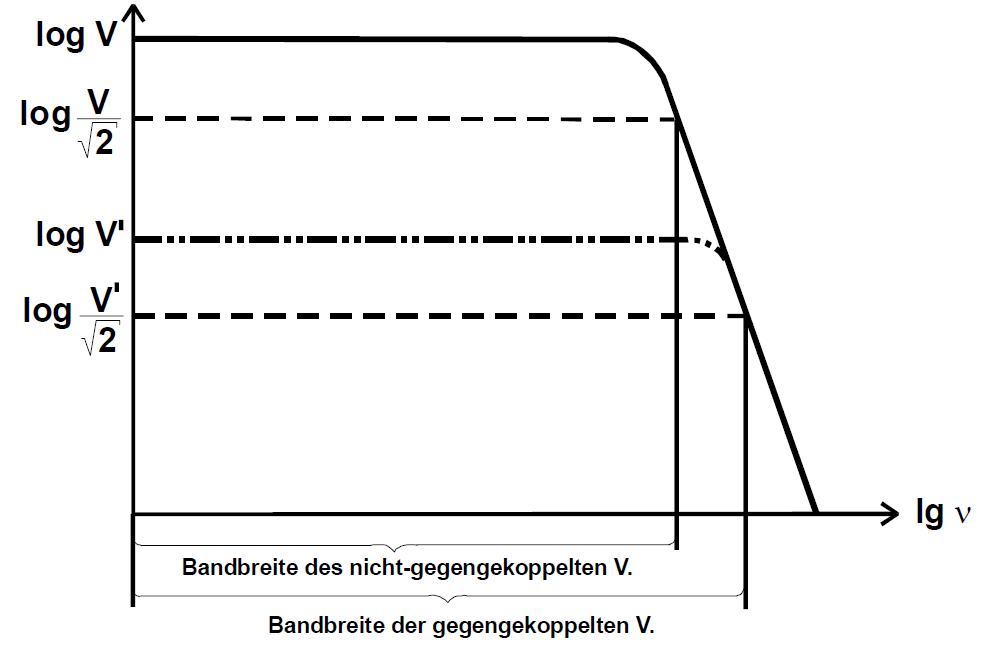
\includegraphics[width=9cm]{images/frequenzgang_operationsverstaerker.png}
\caption{Frequenzgang des Linearverstärkers. [1]}
\label{fig:frequenzgang_operationsverstaerker}
\end{figure}

Der Linearverstärker hat die au"serdem die Funktion eines Tiefpasses. Dies ist in dem folgenden Ersatzschaltbild dargestellt. Damit erklärt sich die Abnahme der Ausgangsamplitude bei großen Frequenzen.
\begin{center}
	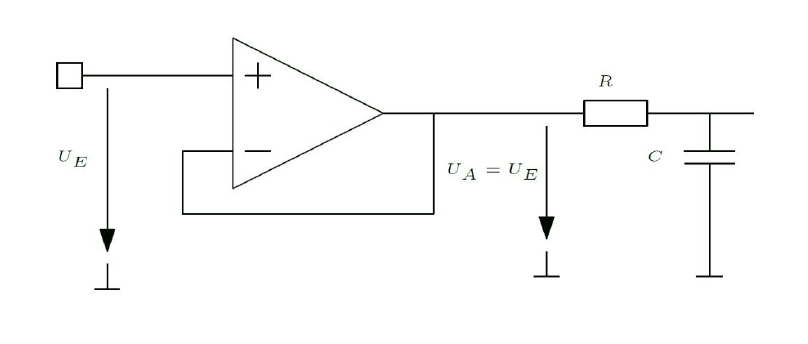
\includegraphics[width=10cm]{images/tiefpass.png}
	\captionof{figure}{Ersatzschaltbild des Tiefpasses}
	\label{fig:tiefpass}
\end{center}
Für den hier vorliegenden RC-Tiefpass ergibt sich mit der Grenzfrequenz $\omega_g$ für den Betrag der Verstärkungsfunktion $V'(\omega)$ sowie die Phase der Verstärkungsfunktion
\begin{align}
|V'(\omega)|=\frac{1}{\sqrt{1+\left(\frac{\omega}{\omega_g}\right)^2}} 
\label{eq:tiefpass}\\
\tan\phi=-\frac{\omega}{\omega_g}\,.
\label{eq:tiefpass_phase}
\end{align} 

\subsubsection{Umkehr-Integrator}
Wird ein Kondensator im Rückkopplungszweig eingebaut, wie in Abbildung \ref{fig:schalplan_umkehrintegrator}, so fungiert die Schaltung als Umkehr-Integrator
\begin{align}
U_\text{A}= \frac{1}{RC}\int dt\ U_1\left(t\right)  \hspace{0.3cm}\text{.}
\end{align}
\begin{figure}[H]
\centering
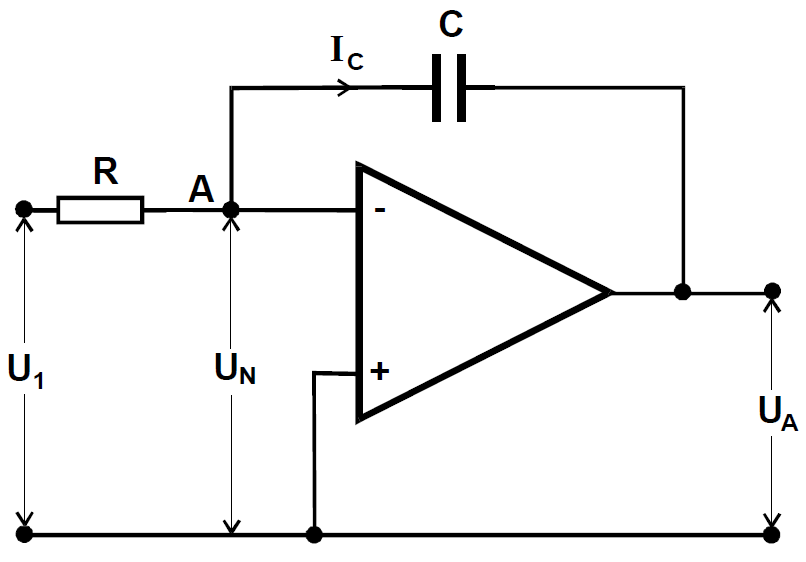
\includegraphics[width=9cm]{images/schalplan_umkehrintegrator.png}
\caption{Schaltplan eines Umkehr-Integrators. [1]}
\label{fig:schalplan_umkehrintegrator}
\end{figure}
Wird beispielsweise eine Sinusspannung 
\begin{align}
U_1=U_0 \sin \omega t
\end{align}
angelegt, so hat das Ausgangssignal die Form
\begin{align}
U_\text{A} = \frac{U_0}{RC\omega}\cos \omega t
\end{align}
und ist somit umgekehrt proportional zur Frequenz des Eingangssignals.
\subsubsection{Umkehr-Differentiator}
Wird der Kondensator anstatt im Rückkopplungszweig vor den invertierten Eingang geschaltet, wie in Abbildung \ref{fig:schalplan_umkehrdifferentiator}, so wirkt die Schaltung als Umkehr-Differentiator
\begin{align}
U_\text{A}= -RC \frac{d}{d t} U_1 \hspace{0.3cm}\text{.}
\end{align}
\begin{figure}[H]
\centering
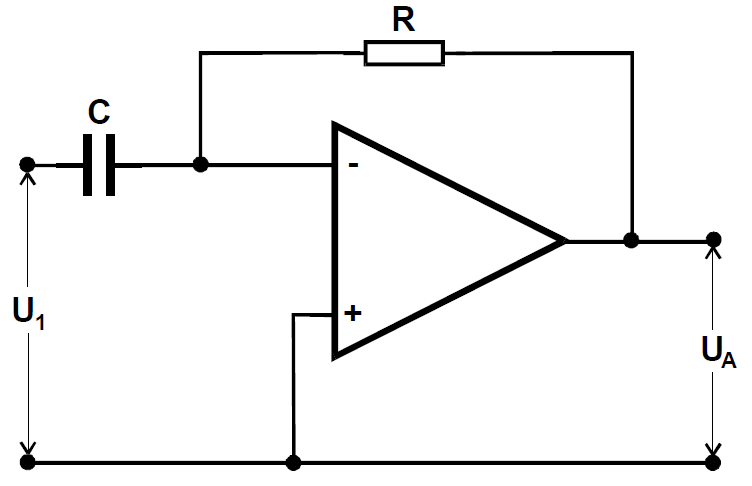
\includegraphics[width=9cm]{images/schaltplan_umkehrdifferentiator.png}
\caption{Schaltplan eines Umkehr-Differentiator. [1]}
\label{fig:schalplan_umkehrdifferentiator}
\end{figure}
Bei einer Sinusspannung
\begin{align}
U_1=U_0 \sin \omega t
\end{align}
kann am Ausgang die Spannung
\begin{align}
U_\text{A} = -RC\omega U_0 \cos \omega t
\end{align}
abgegriffen werden, welche somit proportional zur Frequenz des Eingangssignals ist.
\subsubsection{Schmitt-Trigger}
Bei einem Schmitt-Trigger wird im Gegensatz zum gegengekoppelten invertierenden Linearverstärker die Rückkopplung anstatt auf den invertierenden Eingang auf den nicht-invertierenden Eingang gegeben. Diese Schaltung nach Abbildung \ref{fig:schalplan_schmitt_trigger} fungiert als ein Schalter.

Eine Vergrößerung der Ausgangsspannung führt beim Schmitt-Trigger zu einer Vergrößerung der Eingangsspannung, welche wiederum zu einer Vergrößerung der Ausgangsspannung führt. Diese Schaltung ist instabil, da die Ausgangsspannung spontan auf die Betriebsspannung $U_\text{B}$ springt, wenn die Eingangsspannung $U_1$ den Schwellwert
\begin{align}
U_1=\frac{R_1}{R_\text{P}}U_\text{B}
\end{align} 
überschreitet. Umgekehrt springt die Ausgangsspannung auf die negative Betriebsspannung $-U_\text{B}$, wenn der Schwellwert
\begin{align}
U_1=-\frac{R_1}{R_\text{P}}U_\text{B}
\end{align}
unterschritten wird.
Die Differenz der beiden Umschaltwerte wird als Schalthysterese bezeichnet.
\begin{figure}[H]
\centering
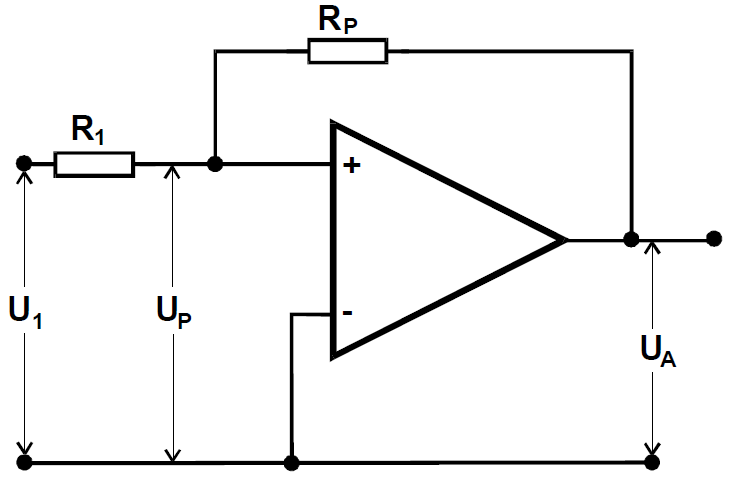
\includegraphics[width=9cm]{images/schaltplan_schmitt_trigger.png}
\caption{Schaltplan eines Schmitt-Triggers. [1]}
\label{fig:schalplan_schmitt_trigger}
\end{figure}


\subsubsection{Der Operationsverstärker als Signalgenerator}
Mit Hilfe der in den vorherigen Abschnitten beschriebenen Schaltungen lässt sich ein Rechteck- und Dreiecksgenerator erzeugen. 
Es wird dabei jeweils ein Schmitt-Trigger und ein Integrator benötigt, die wie in Abbildung \ref{fig:schalplan_generator} geschaltet werden.

Der Schmitt-Trigger liefert eine konstante Ausgangsspannung $U_\text{B}$, die anschließend vom Integrator integriert wird. Es fällt somit die Ausgangsspannung $U_1$ linear ab, bis sie den Schwellwert des Triggers erreicht und dieser auf $-U_\text{B}$ springt. Diese wird nun weiter integriert und steigt durch das invertierte Vorzeichen von $U_\text{B}$ wieder an.
Daraus ergibt sich eine periodische Schwingung, die ihre Extrema an den Schwellwerten des Schmitt-Triggers besitzt. Die Frequenz ist von der Integratorzeitkonstanten und den Widerständen der Mittelkopplung abhängig.
\begin{figure}[H]
\centering
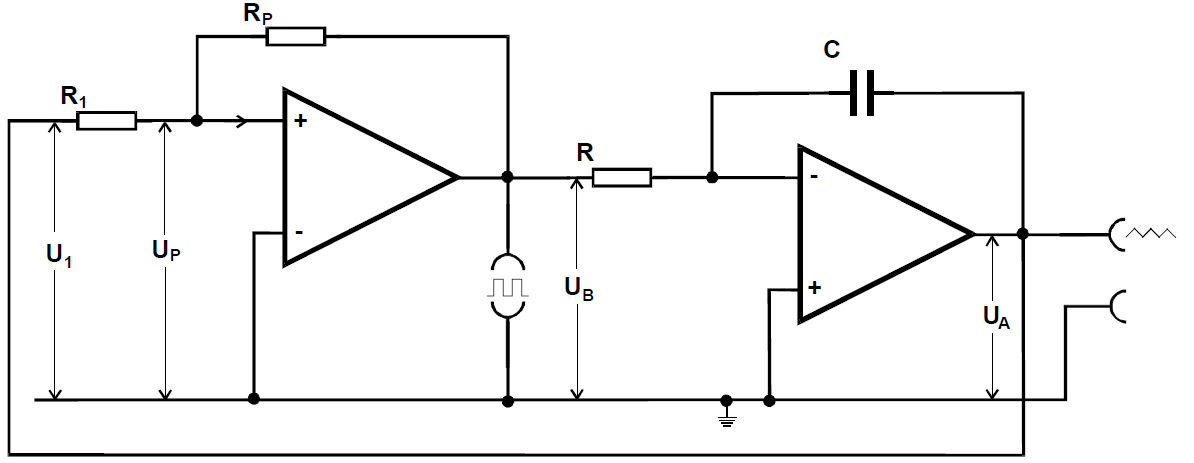
\includegraphics[width=13.0cm]{images/schaltplan_generator.png}
\caption{Schaltplan eines Rechteck-/Dreieckgenerators. [1]}
\label{fig:schalplan_generator}
\end{figure}

\subsubsection{Erzeugung amplitudenmodulierter Sinusschwingung}
Eine Sinusschwingung mit zeitlich veränderlicher Amplitude lässt sich durch zwei Integratoren und einen Umkehrverstärker realisieren, wie in Abbildung \ref{fig:schalplan_schwingung} dargestellt.
Die Schaltung kann durch die Differentialgleichung
\begin{align}
\frac{d^2 U_\text{A}}{dt^2}-\frac{\eta}{10 RC} \frac{d U_\text{A}}{dt}+\frac{U_\text{A}}{R^2C^2}=0
\end{align}
beschrieben werden. Die Lösung 
\begin{align}
U_\text{A}\left(t\right)=U_0\exp \left(\frac{\eta t}{20 RC}\right)\sin \frac{t}{RC}
\end{align}
beschreibt eine gedämpfte ($\eta < 0$) bzw. entdämpfte Sinusschwingung. Dabei ist die Schwingungsdauer
\begin{align}
T=2\pi RC
\label{eq:freqsin}
\end{align}
und die Abklingdauer
\begin{align}
\tau=\frac{20RC}{\left|\eta \right| }\hspace{0.3cm}\text{.}
\label{eq:key}
\end{align}
\begin{figure}[H]
\centering
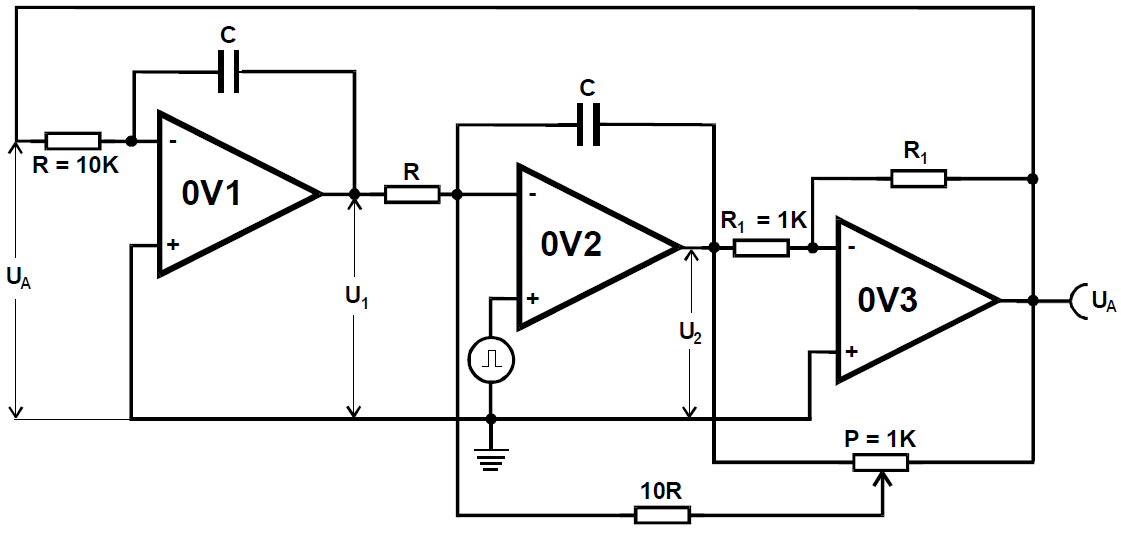
\includegraphics[width=13cm]{images/schaltplan_schwingung.png}
\caption{Schaltplan einer linearen Schwingungsdifferentialgleichung mit zeitlich veränderlichen Amplitude. [1]}
\label{fig:schalplan_schwingung}
\end{figure}


\newpage

\section{Durchführung}

\subsection{Frequenzgang und Phasenbeziehung des gegengekoppelten Verstärkers}
Ein gegengekoppelter Verstärker wird aufgebaut und bei vier verschiedenen Verstärkungen V' wird der entsprechende Frequenzgang vermessen. Au"serdem wird die Phasenbeziehung zwischen Ausgangs- und Eingangsspannung bei einer aufgeführten Verstärkung V' vermessen.

\subsection{Der Umkehrintegrator- und Differentiator}
Ein Umkehrintegrator und -differentiator werden aufgebaut und die Beziehung $U_A\propto\frac{1}{\omega}$ bzw. $U_A\propto\omega$ zwischen Ausgangsspannung $U_A$ und Frequenz $\omega$ wird überprüft. Au"serdem werden eine Sinus-, eine Rechteck- und eine Dreiecksspannung auf den Umkehrintegrator und -differentiator gegeben und von den Ausgangssignalen Bilder erstellt.

\subsection{Der Schmitt-Trigger}
Ein Schmitt-Trigger wird aufgebaut und der Scheitelwert der Spannung sowie die Betriebsspannung gemessen.

\subsection{Der Dreiecksgenerator}
Ein Dreieckgenerator wird aufgebaut und ein Bild der erzeugten Spannung aufgenommen. Desweiteren werden Amplitude und Frequenz des Ausgangssignals ermittelt.

\subsection{Die Schwingungsdifferentialschaltung}
Mithilfe einer Schwingungsdifferentialschaltung wird eine ungedämpfte und eine gedämpfte Sinusspannung erzeugt. Davon werden Bilder aufgenommen und die Abklingdauer der gedämpften Schwingung bestimmt.

\section{Auswertung}

\subsection{Frequenzgang und Phasengang des gegengekoppelten Verstärkers}

In Abbildung \ref{fig:frequenzgang} sind die Frequenzgänge des gegengekoppelten Verstärkers für verschiedene Verstärkungsgrade $V'$ dargestellt. Dazu wurde jeweils eine konstante Funktion, die die Verstärkungsfunktion bei der Grenzfrequenz $f_g$ schneidet und den konstanten Wert $\frac{V'}{\sqrt{2}}$ hat, sowie ein linearer Fit für alle Werte von $f>f_g$ angefertigt. Der lineare Ansatz, der sich aus Gleichung \ref{eq:tiefpass} sowie der Näherung $f \gg f_g$ ergibt, lautet
\begin{align}
\ln(|V'(\omega)|)=-m\ln(f)+\ln(f_g)\,.
\end{align} 
Es wurde dabei stets ein Widerstand der Grö"se $R_1=\SI{1}{\kilo\ohm}$ verwendet. Die Tabellen mit den Messdaten sind im Anhang zu finden.\\
\begin{minipage}[t]{0.6\textwidth}
		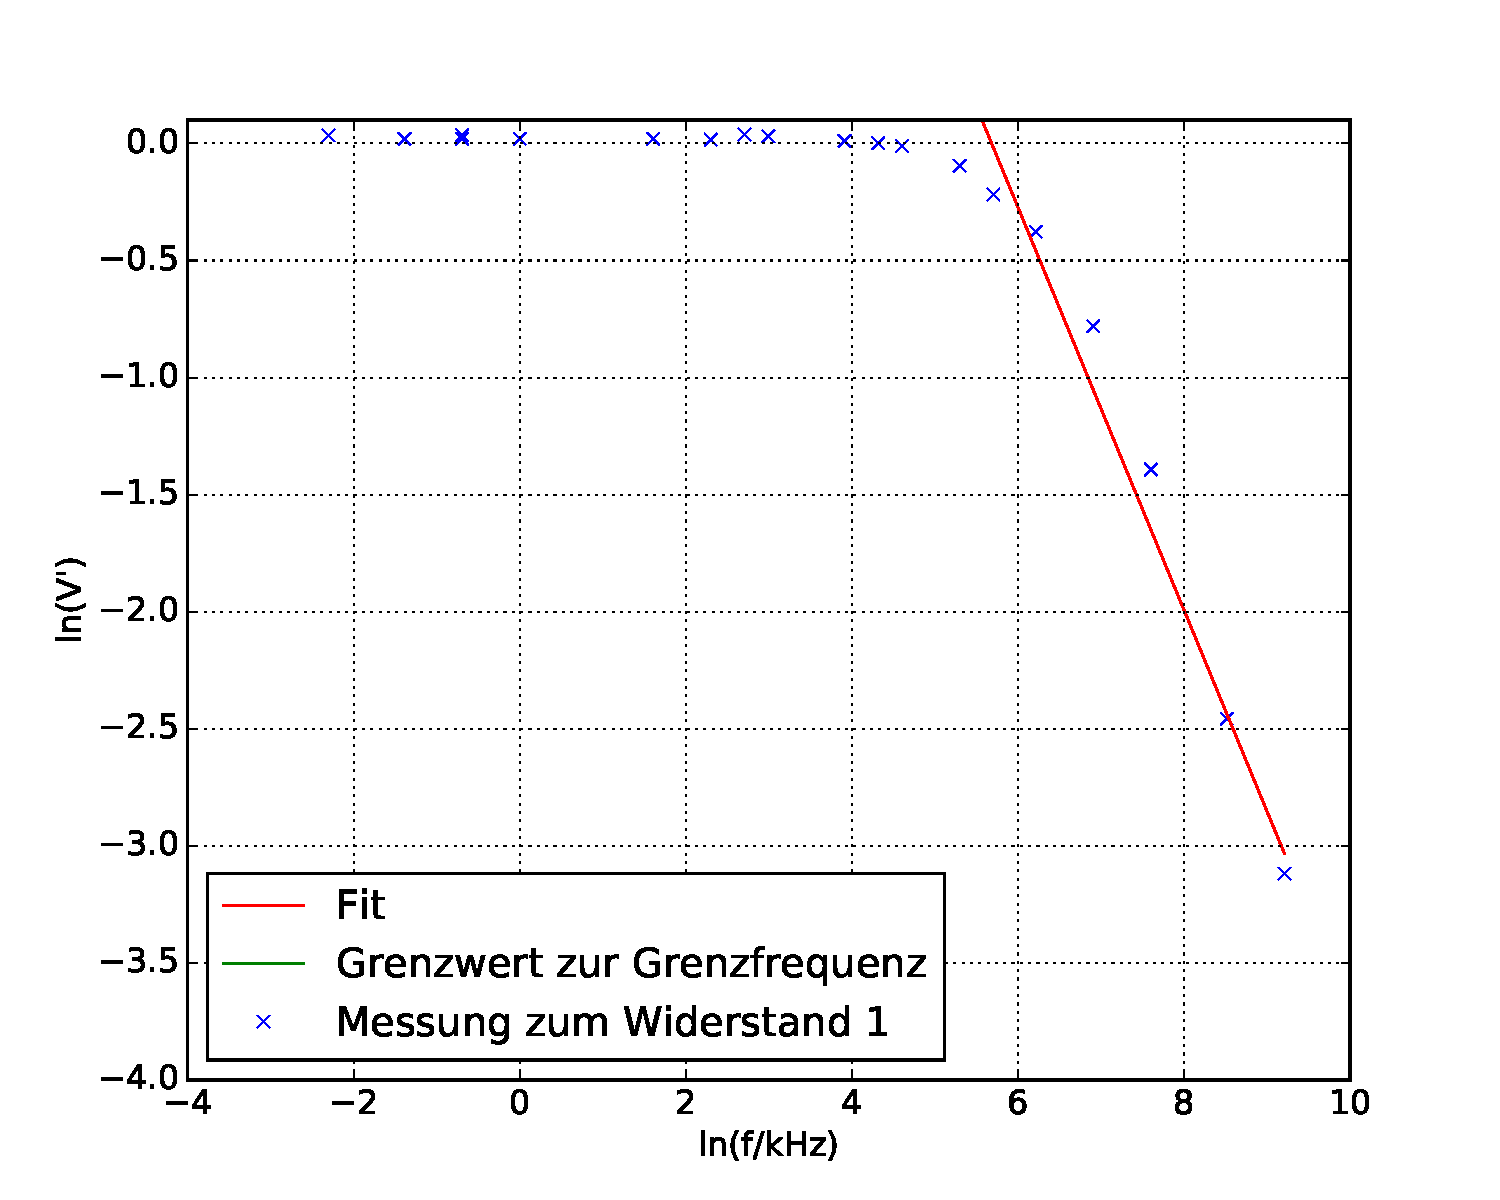
\includegraphics[width=\textwidth]{images/plot1.pdf}
		\centering
		a)
\end{minipage}
\begin{minipage}[t]{0.6\textwidth}
		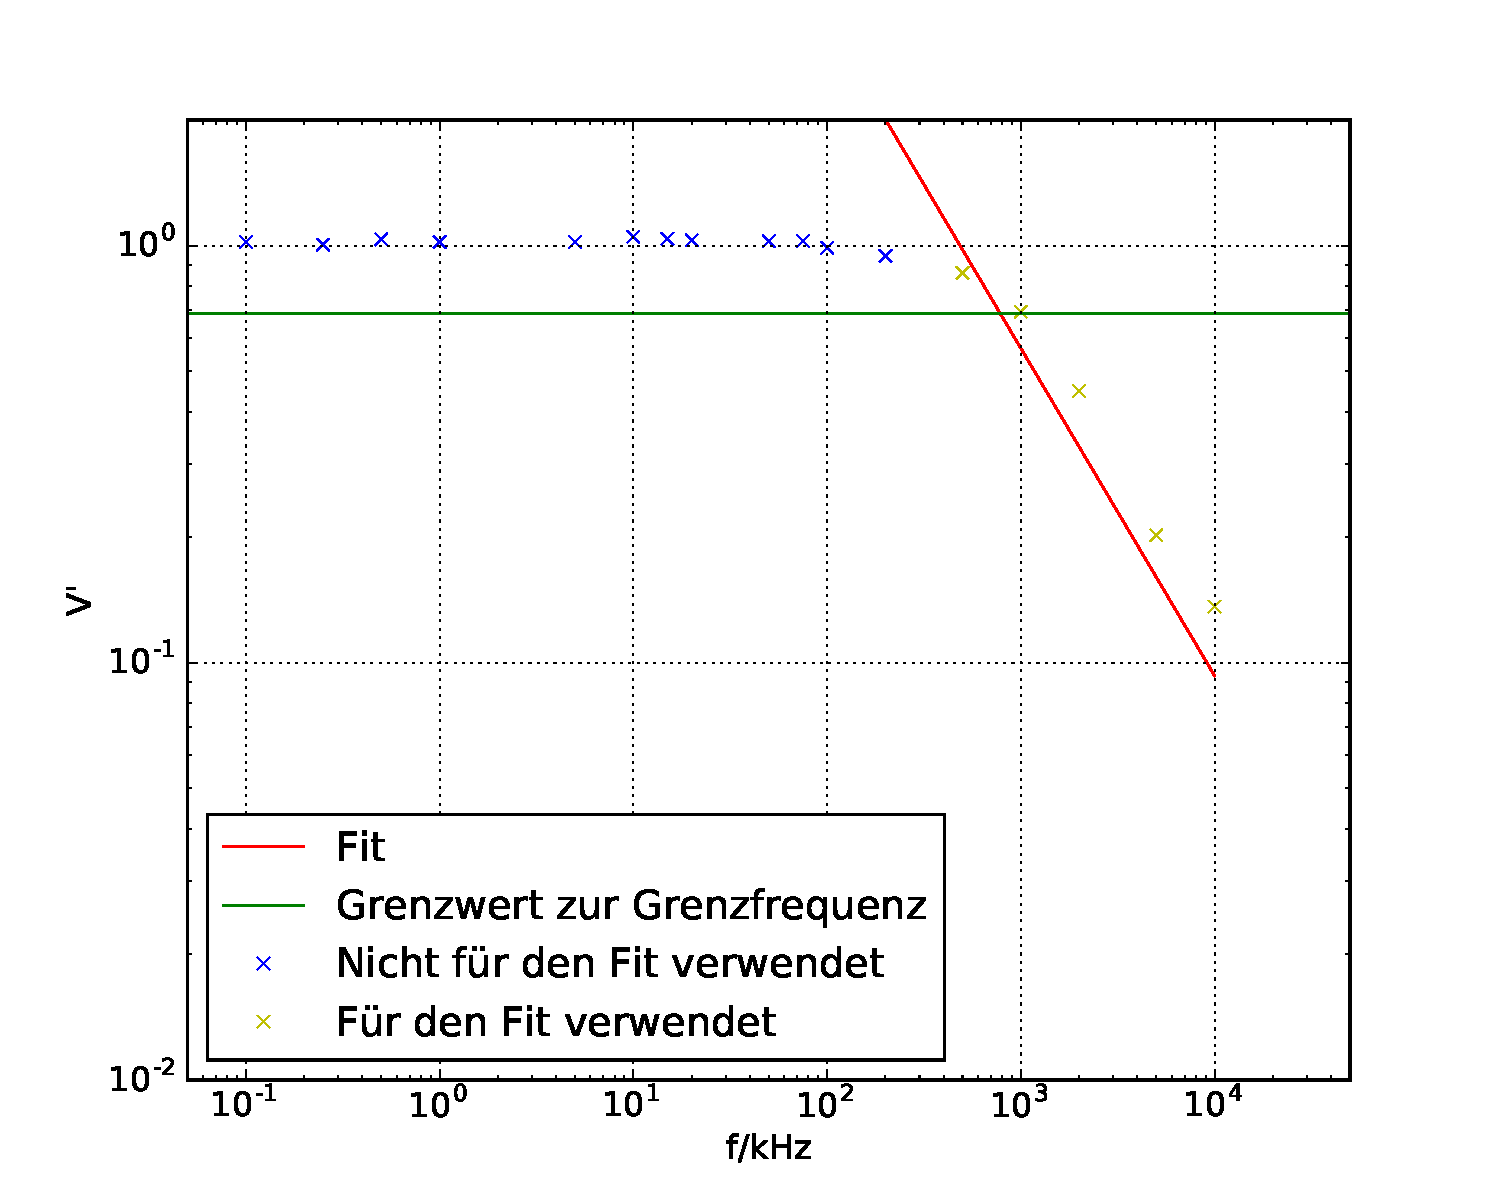
\includegraphics[width=\textwidth]{images/plot2.pdf}
		\centering
		b)
\end{minipage} \\
\begin{minipage}[t]{0.6\textwidth}
		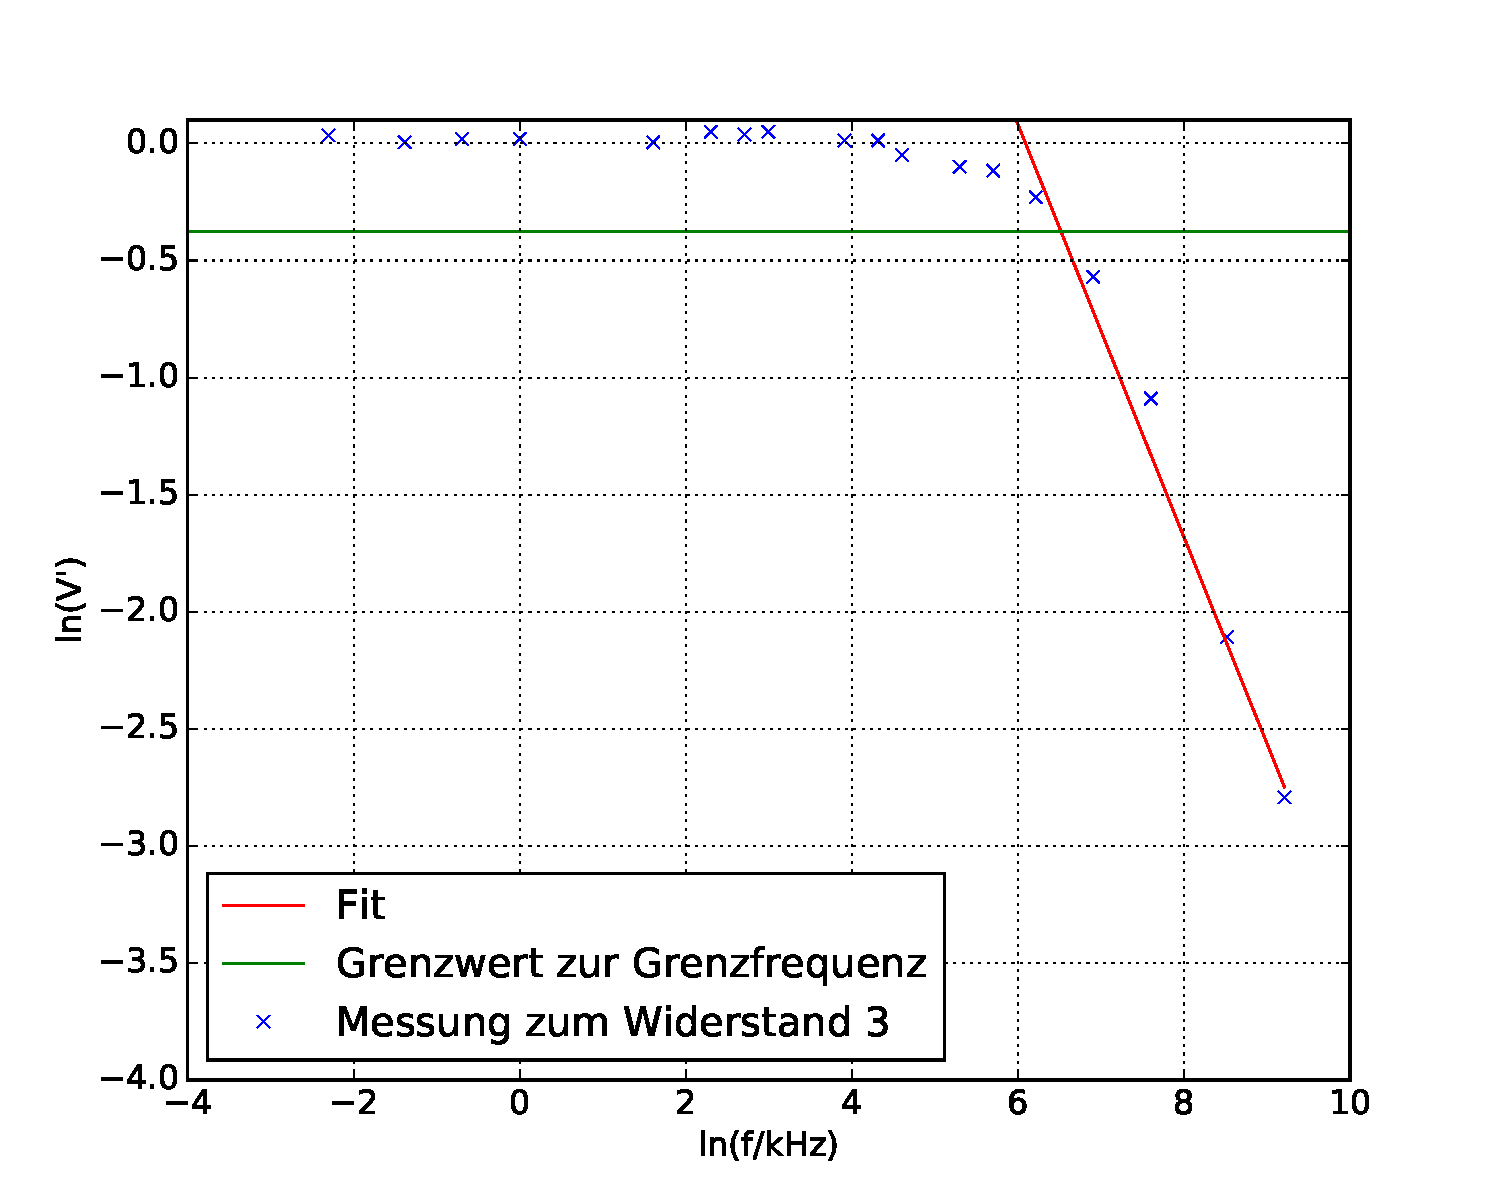
\includegraphics[width=\textwidth]{images/plot3.pdf}
		\centering
		c)
\end{minipage}
\begin{minipage}[t]{0.6\textwidth}
		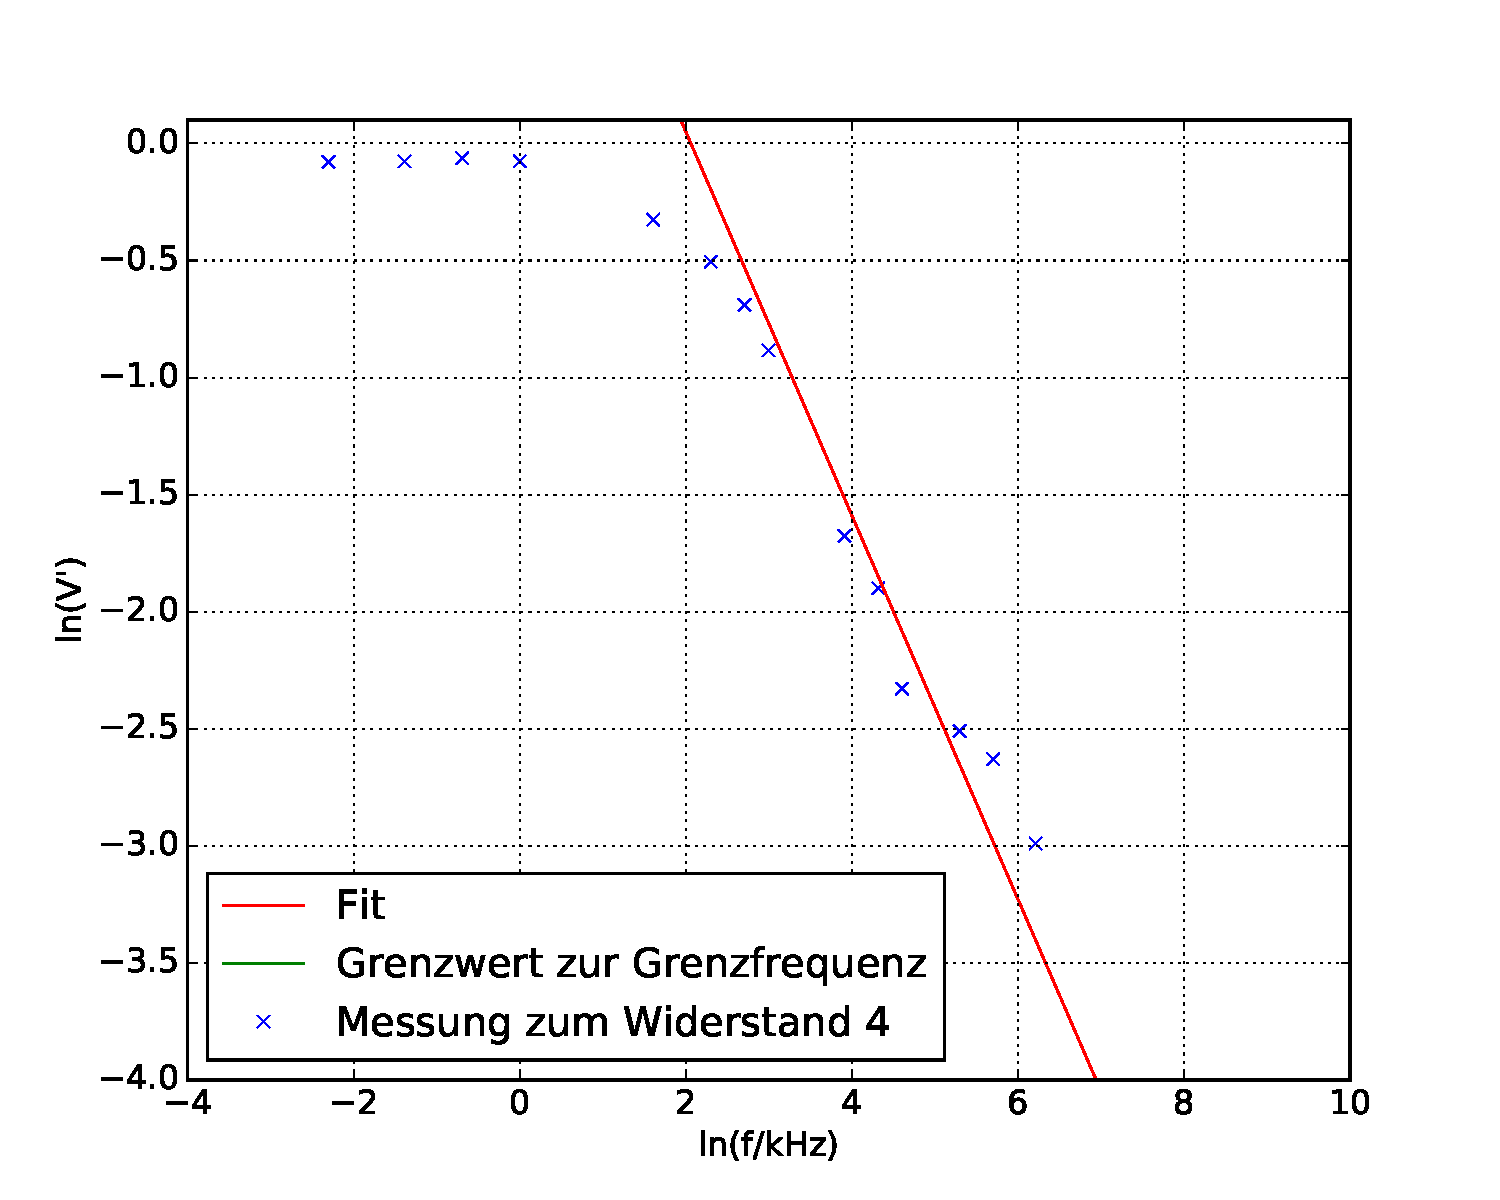
\includegraphics[width=\textwidth]{images/plot4.pdf}
		\centering
		d)
\end{minipage}
\captionof{figure}{Frequenzgang für $R_n=$ a) $\SI{1}{\kilo\ohm}$, b) $\SI{100}{\ohm}$, c) $\SI{570}{\ohm}$, d) $\SI{570}{\ohm}$}
\label{fig:frequenzgang}
\vspace{0.5cm}
In Tabelle \ref{tab:frequenzgang} sind die Grenzfrequenz $f_g$, die Verstärkung in Theorie 	$V'_{\text{ideal}}$, die sich aus Gleichung \ref{eq:verstaerkung_ideal} ergibt, und Experiment $V'_{\text{exp}}$, die sich aus dem Mittelwert der blau markierten Daten ergibt, die Leerlaufverstärkung $V_\text{Leerlauf}$, die sich aus Gleichung \ref{eq:leerlaufkorrektur} ergibt, die Steigung m und das Verstärkungs-Bandbreite-Produkt $B_0v_0=\frac{V'}{\sqrt{2}}f_g$ für die einzelnen verwendeten Widerstände dargestellt. \\
\begin{table}[H]
	\centering
		\captionof{table}{Experimentell bestimmte Kenndaten}
		\label{tab:frequenzgang}
		\hskip-1.50cm\begin{tabular}{r r r r r}
			\toprule
				Kenngrö"se & $R_n=\SI{1}{\kilo\ohm}$ & $R_n=\SI{100}{\ohm}$ &  $R_n=\SI{570}{\ohm}$ & $R_n=\SI{100}{\kilo\ohm}$ \\
			\midrule
				$f_{\text{g}}$ [kHz] & $450 \pm 350$ & $1000 \pm 500$ & $700 \pm 500$ & $14 \pm 11$ \\
				$V'_{\text{ideal}}$ & $1.0$ & $0.1$ & $0.57$ & $100$ \\
				$V'_{\text{exp}}$ & $0.980 \pm 0.007$ & $0.970 \pm 0.012$ & $0.970 \pm 0.012$ & $0.884 \pm 0.006$ \\
				$V_{\text{Leerlauf}}$ & $48.25 \pm 17.04$ & $-0.111 \pm 0.000$ & $-1.38 \pm 0.02$ & $0.892 \pm 0.006$ \\
				m & $-0.860 \pm 0.070$ & $-0.897 \pm 0.046$ & $-0.882 \pm 0.070$ & $-0.819 \pm 0.098$\\
				$B_0v_0$ [kHz] & $441.58 \pm 347.37$ & $955.89 \pm 525.67$ & $658.61 \pm 529.53$ & $12.33 \pm 9.51$ \\
			\bottomrule
		\end{tabular}
\end{table}

In Abbildung \ref{fig:phase} sind die Messwerte für die Phasenverschiebung zwischen Eingangs- und Ausgangsspannung dargestellt.Die entsprechenden Messwerte sind in Tabelle \ref{tab:phase} zu finden.
\begin{center}
	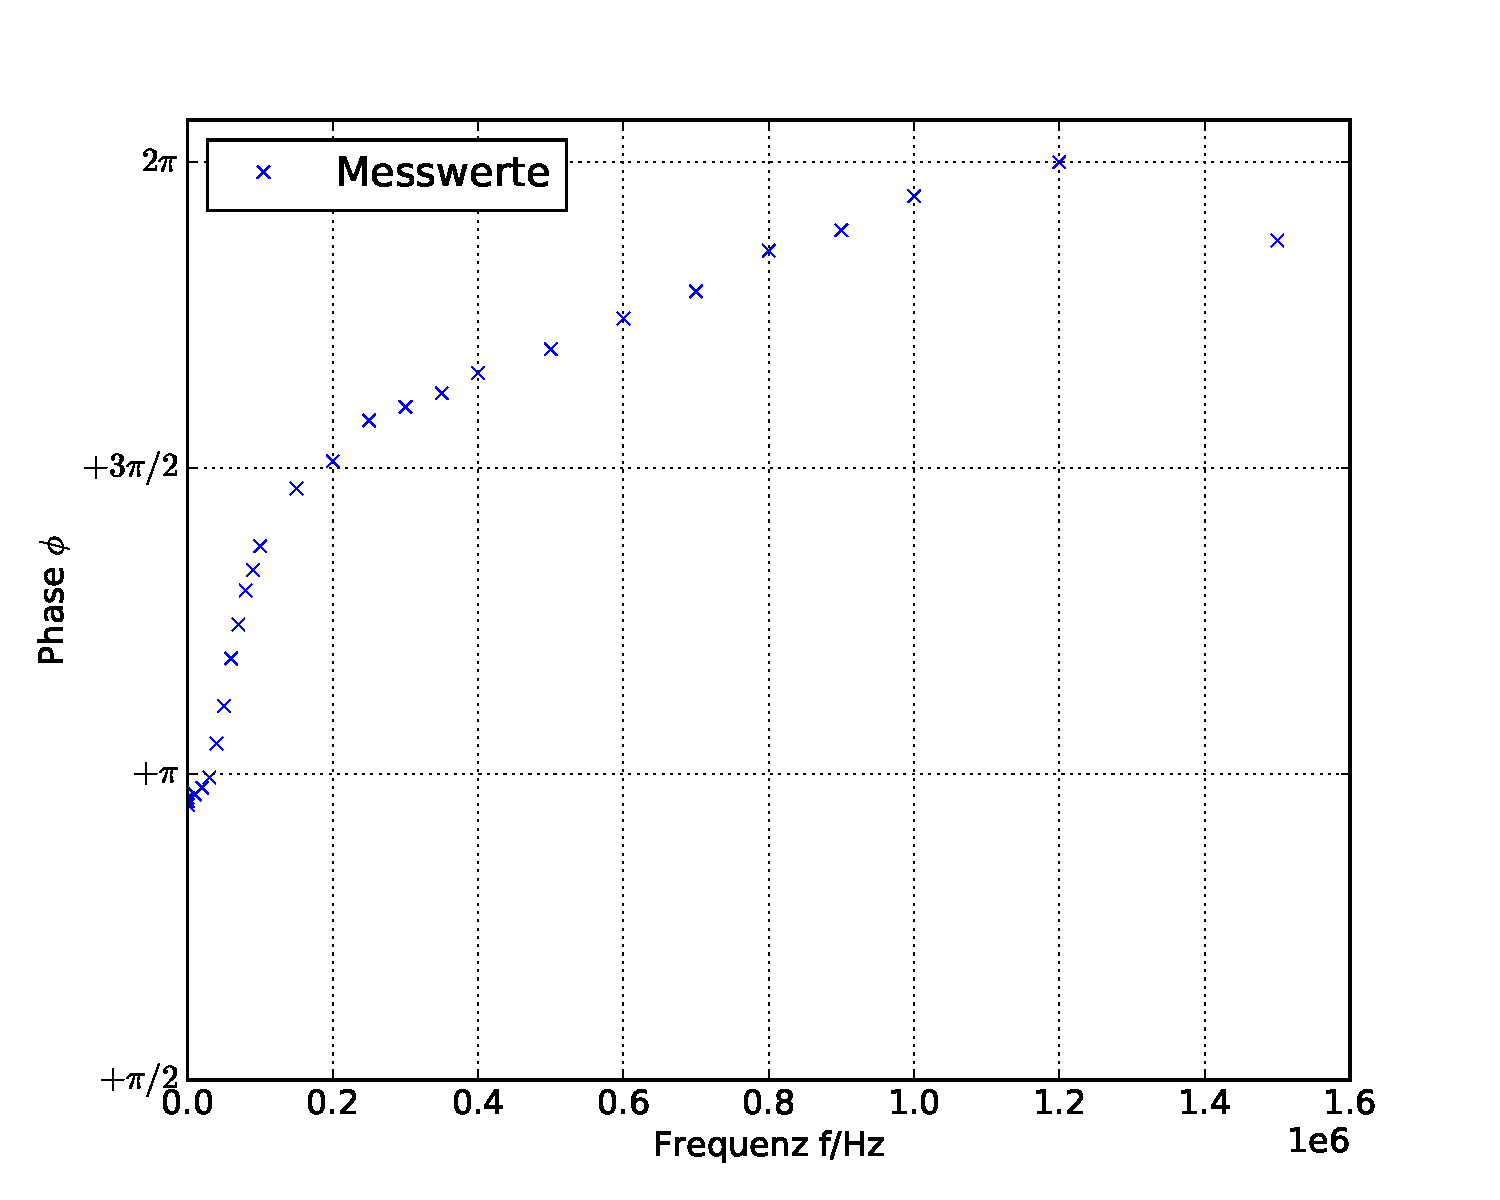
\includegraphics[width=10cm]{images/phase_frequenz.pdf}
	\captionof{figure}{Phasenverschiebung zwischen Eingangs- und Ausgangsspannung aufgetragen gegen die Fequenz}
	\label{fig:phase}
\end{center}

\subsection{Der Umkehrintegrator und -differentiator}
Für den Aufbau des Umkehrintegrators wurden ein Widerstand $R=\SI{32.7}{\kilo\ohm}$ und eine Kapazität $C=\SI{13.6}{\nano\farad}$ verwendet. Die gemessenen Ausgangsspannungen in Abhängigkeit von der Frequenz sind in Tabelle \ref{tab:integrator} dargestellt, in Abbildungen \ref{fig:sinusint}-\ref{fig:dreieckint} sind die Thermodrucke des Ausgangssignals für verschiedene Eingangssignalformen dargestellt. \\
Es wird eine lineare Ausgleichsrechnung der Form 
\begin{align}
\ln |U_A| = \ln\left(\frac{U_0}{RC}\right)+m\cdot\omega
\end{align}
gemacht. \\
Mithilfe der linearen Ausgleichsrechnung ergibt sich die Steigung $m$ zu
\begin{align*}
m = -0.754\pm 0.040\,.
\end{align*}
\begin{center}
	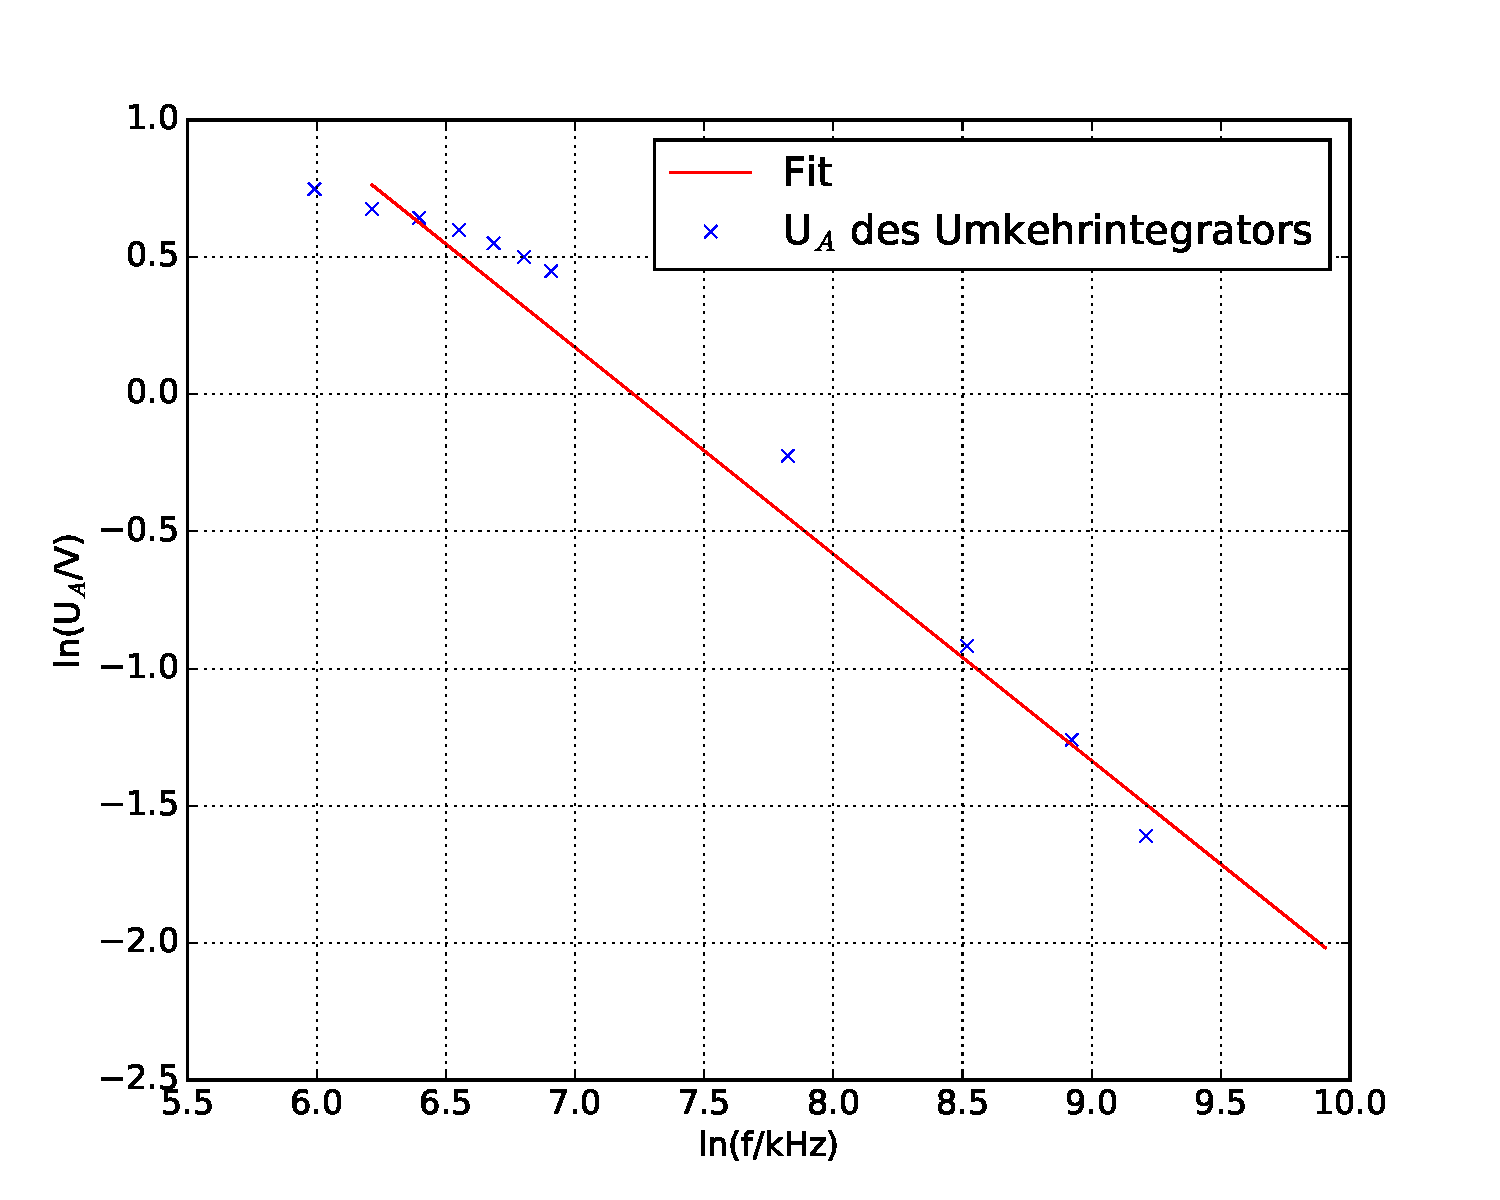
\includegraphics[width=12cm]{images/integrator.pdf}
	\captionof{figure}{Ausgangsspannung $U_A$ des Umkehrintegrators bei variierter Frequenz $f$}
	\label{fig:integrator}
\end{center}
\begin{minipage}[t]{0.5\textwidth}
	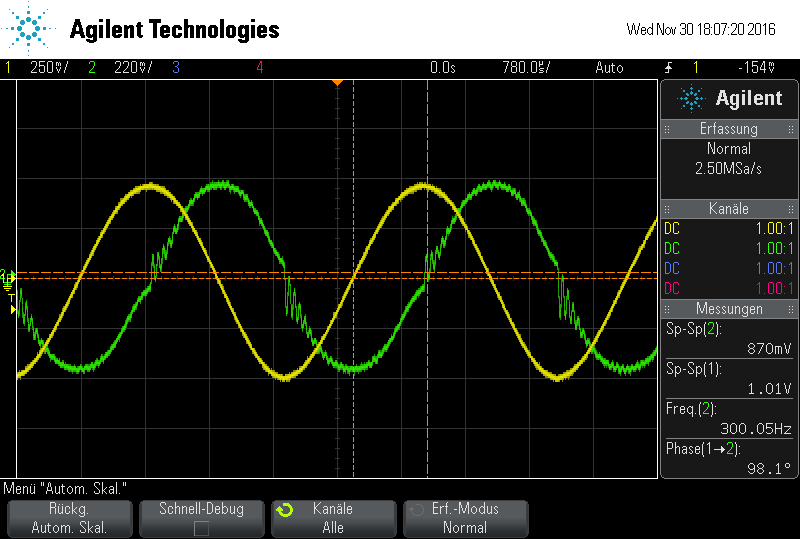
\includegraphics[width=\textwidth]{images/sinus_int}
	\captionof{figure}{Gelbes Sinus-Signal: $U_E$, grünes negatives Cosinus-Signal: $U_A$}
	\label{fig:sinusint}
\end{minipage}
\hspace{0.1\textwidth}
\begin{minipage}[t]{0.5\textwidth}
	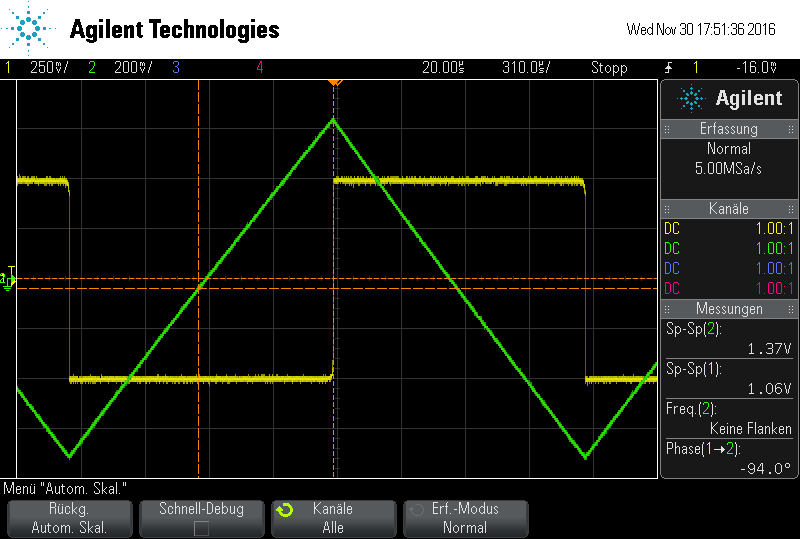
\includegraphics[width=\textwidth]{images/rechteck_int}
	\captionof{figure}{Gelbes Rechteck-Signal: $U_E$, grünes Dreieck-Signal: $U_A$}
	\label{fig:rechteckint}
\end{minipage} \\
\begin{minipage}[t]{0.5\textwidth}
	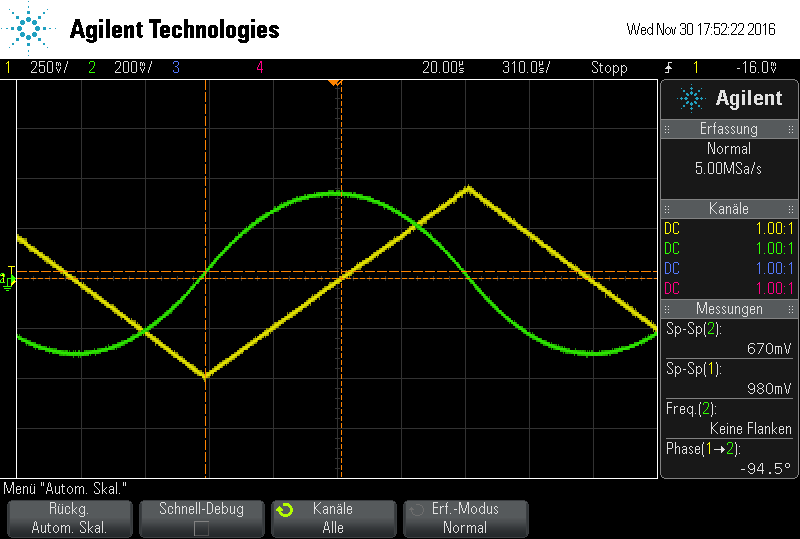
\includegraphics[width=\textwidth]{images/dreieck_int}
	\captionof{figure}{Gelbes Dreick-Signal: $U_E$, grünes Parabel-Signal: $U_A$}
	\label{fig:dreieckint}
\end{minipage} \\
Für den Aufbau des Umkehrdifferentiators wurden ein Widerstand $R=\SI{32.7}{\kilo\ohm}$ und eine Kapazität $C=\SI{13.6}{\nano\farad}$ verwendet. Die gemessenen Ausgangsspannungen in Abhängigkeit von der Frequenz sind in Tabelle \ref{tab:differentiator} dargestellt, in Abbildungen \ref{fig:sinusdiff}-\ref{fig:dreieckdiff} sind die Thermodrucke des Ausgangssignals für verschiedene Eingangssignalformen dargestellt.
Es wird eine lineare Ausgleichsrechnung der Form 
\begin{align}
\ln |U_A| = \ln\left(-RCU_0\right)+m\cdot\omega
\end{align}
gemacht. \\
Mithilfe der linearen Ausgleichsrechnung ergibt sich die Steigung $m$ zu
\begin{align*}
m = -0.797 \pm 0.039\,.
\end{align*}
\begin{center}
	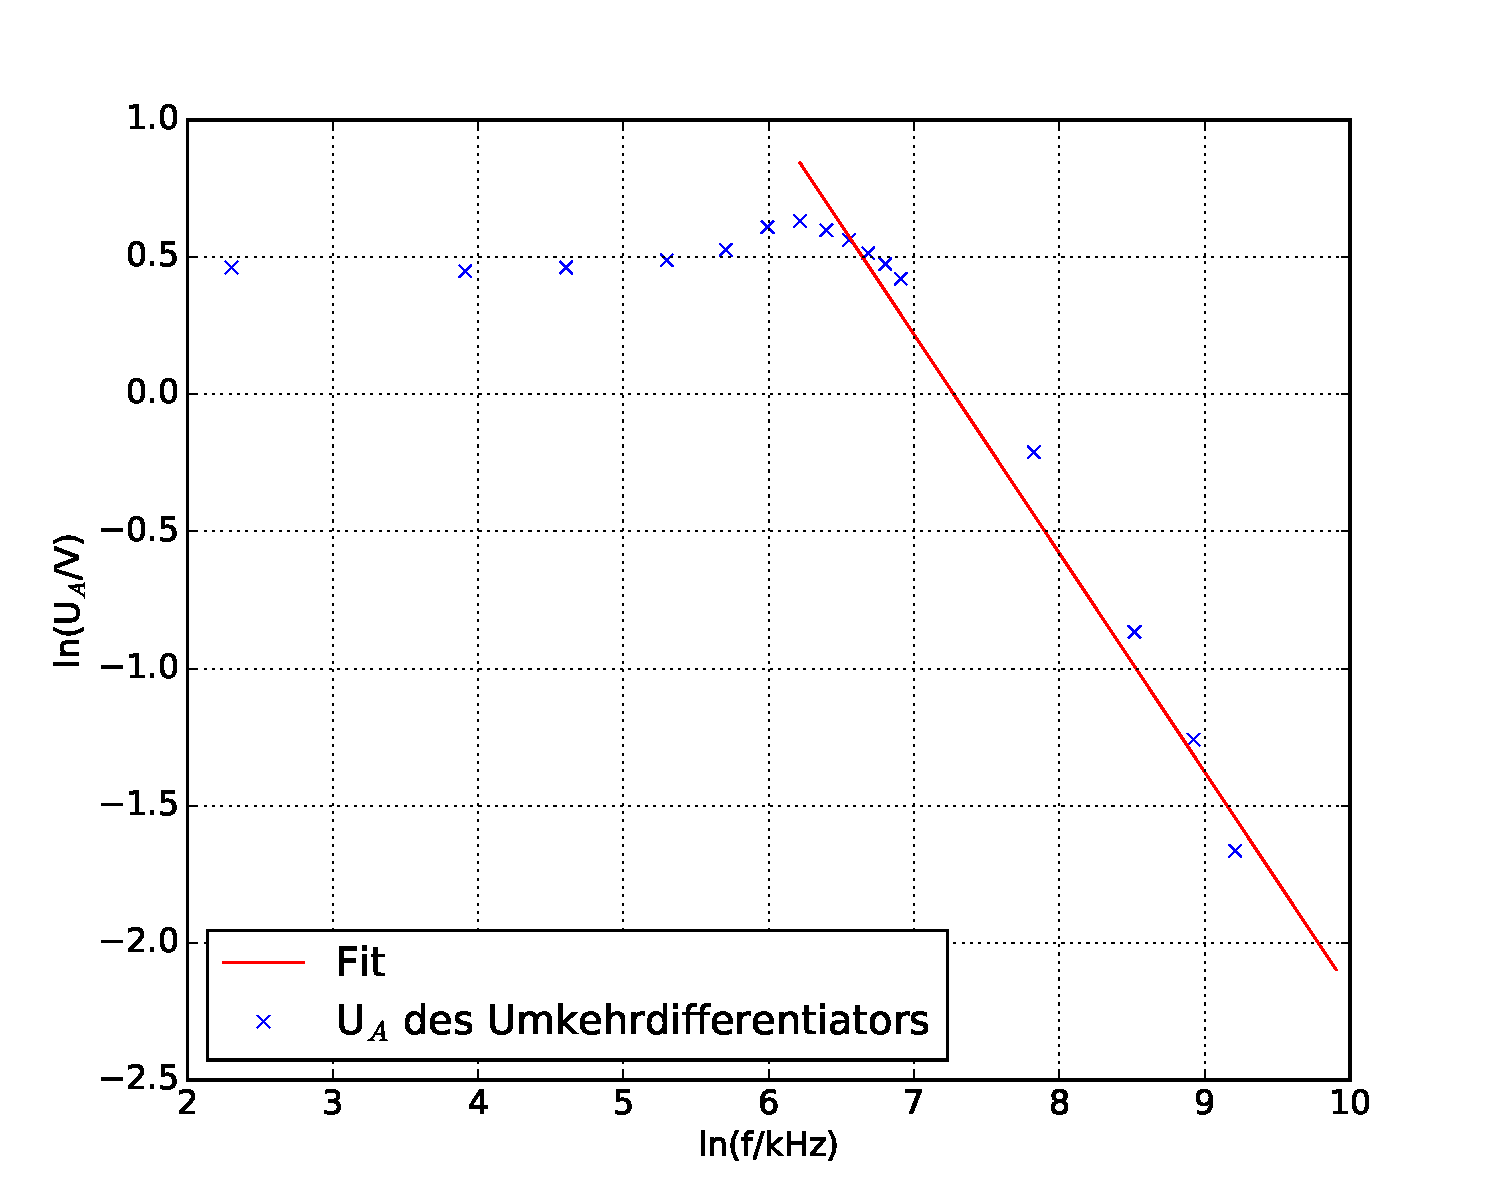
\includegraphics[width=12cm]{images/differentiator.pdf}
	\captionof{figure}{Ausgangsspannung $U_A$ des Umkehrdifferentiators bei variierter Frequenz $f$}
	\label{fig:differentiator}
\end{center}
\begin{minipage}[t]{0.5\textwidth}
	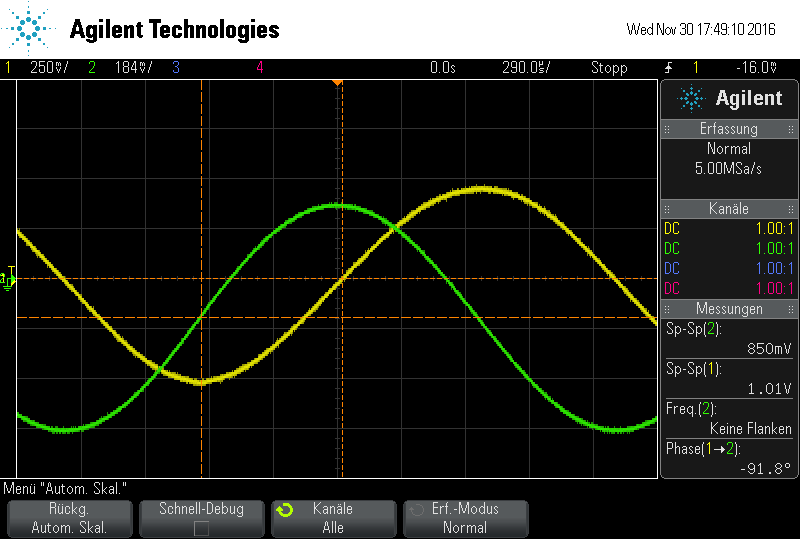
\includegraphics[width=\textwidth]{images/sinus_diff}
	\captionof{figure}{Grünes Sinus-Signal: $U_E$, gelbes Cosinus-Signal: $U_A$}
	\label{fig:sinusdiff}
\end{minipage}
\hspace{0.1\textwidth}
\begin{minipage}[t]{0.5\textwidth}
	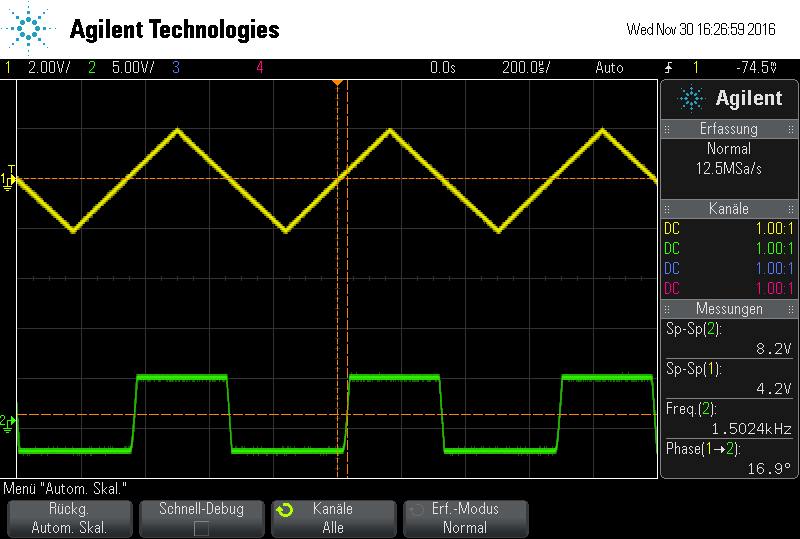
\includegraphics[width=\textwidth]{images/rechteck_diff}
	\captionof{figure}{Grünes Rechteck-Signal: $U_E$, gelbes Dreieck-Signals: $U_A$}
	\label{fig:rechteckdiff}
\end{minipage} \\
\begin{minipage}[t]{0.5\textwidth}
	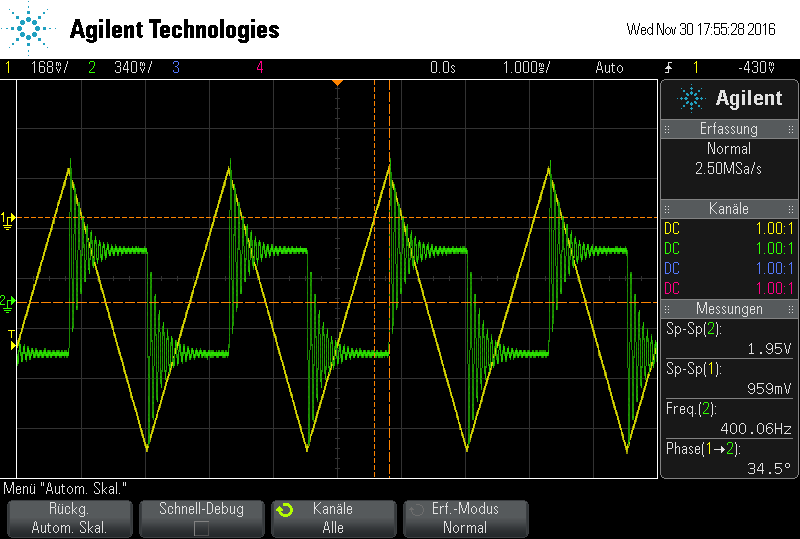
\includegraphics[width=\textwidth]{images/dreieck_diff}
	\captionof{figure}{Gelbes Dreieck-Signal: $U_E$, grünes Rechteck-Signal: $U_A$}
	\label{fig:dreieckdiff}
\end{minipage} 

\subsection{Der Schmitt-Trigger}
Für den Aufbau des Schmitt-Triggers wurden die Widerstände $R_P=\SI{33}{\kilo\ohm}$ und $R_1=\SI{100}{\ohm}$ verwendet. Der Wert des Betriebsspannung betrug $U_B=\SI{13.08}{\volt}$. Dazu ist anzumerken, dass $U\ll U_B=\SI{13.08}{\volt}$ ist. Der Signalverlauf ist in Abbildung \ref{fig:schmitt} dargestellt.\\
\begin{center}
	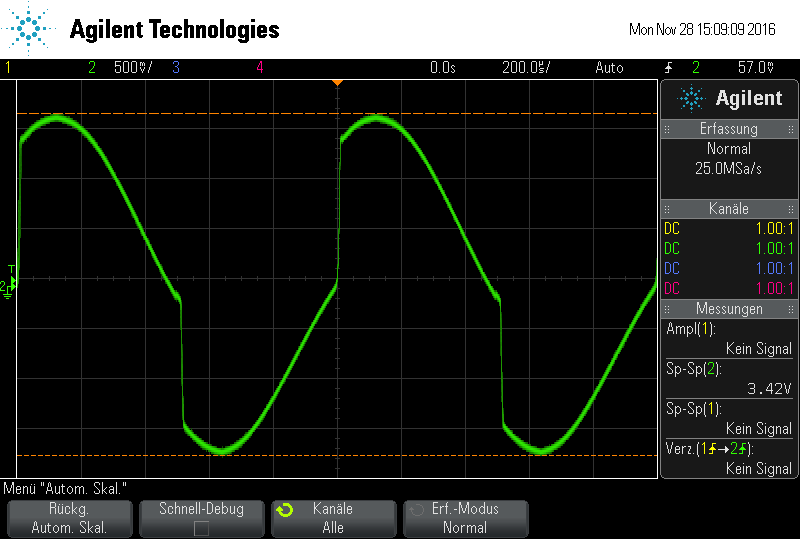
\includegraphics[width=10cm]{images/schmitt.png}
	\captionof{figure}{Signalverlauf der Ausgangsspannung des Schmitt-Triggers}
	\label{fig:schmitt}
\end{center}
Der Kippspannung betrug $U_{kipp}=\SI{90}{\milli\volt}$ die theoretisch errechnete Kippspannung betrug
\begin{align*}
U_{theor}=\SI{39.6}{\milli\volt}\,.
\end{align*}

\subsection{Der Dreiecksgenerator}
Der Dreieckgenerator wurde mit der Konfiguration
\begin{align*}
R_1=\SI{100}{\ohm}, && R_P=\SI{33}{\kilo\ohm}, && R=\SI{10}{\kilo\ohm} && \text{und} && C=\SI{100}{\nano\farad}
\end{align*}
aufgebaut. Die Betriebsspannung wurde auf $U_B=\SI{13.08}{\volt}$ eingestellt. Auf dem Oszilloskop wird ein Signal mit zwei unterschiedlichen Extremwerten beobachtet. Das Maximum befindet sich bei $U_{\text{max}}=\SI{0.69}{\volt}$, das Minimum bei $U_{\text{min}}=\SI{-0.85}{\volt}$.
Der Signalverlauf ist in Abbildung \ref{fig:dreieckgen} dargestellt.
\begin{center}
	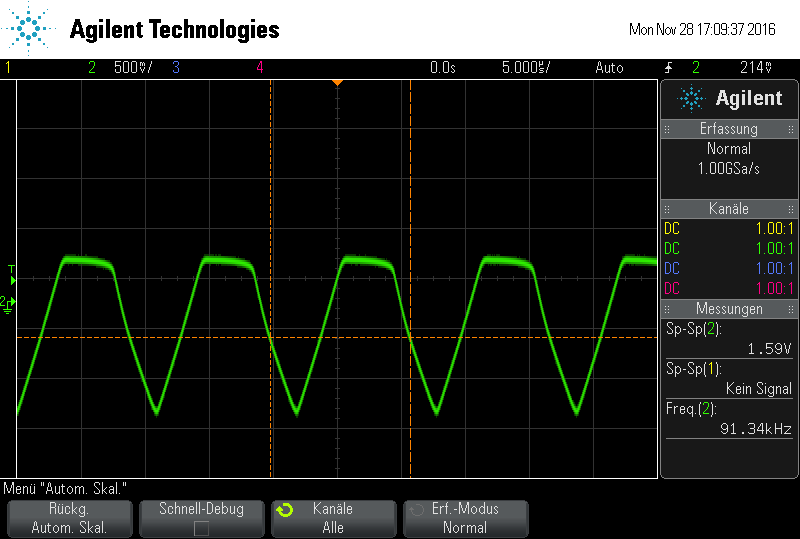
\includegraphics[width=10cm]{images/dreieckgen.png}
	\captionof{figure}{Signalverlauf der Ausgangsspannung des Dreiecksgenerators}
	\label{fig:dreieckgen}
\end{center}
Die Zeit, um den Kondensator vollständig aufzuladen, beträgt $T_ {1/2}=2RC$, für eine ganze Periode daher $T=2RC$. Die Frequenz ist desweiteren proportional zur Verstärkung. \\
Die theoretische Frequenz des Dreiecksgenerators ergibt sich daher zu
\begin{align}
f_{theo}=\frac{R_P}{4R_1RC}\,.
\end{align}
Somit ergaben sich für diese Konfiguration folgende Werte:
\begin{align}
f_{theo}=\SI{82.5}{\kilo\hertz} &  & f_{exp}=\SI{91.34}{\kilo\hertz}\,.
\end{align}

\subsection{Die Schwingungsdifferentialschaltung}
Für die Kapazität in der Schwingungsdifferentialschaltung wurden $R=\SI{10}{\kilo\ohm}$ und \\ $C=\SI{22.5}{\nano\farad}$ gewählt. \\
Die theoretischen Werte für die Frequenz $f_{theo}$ und die Abklingdauer $\tau$ ergeben sich gemä"s Gleichungen \ref{eq:freqsin} und \ref{eq:key} zu
\begin{align}
f_{theo} = \frac{1}{2\pi RC}=\SI{723.43}{\hertz} \\
\tau = 20RC=\SI{4.5}{\milli\second}\,.
\end{align}
In Abbildung \ref{fig:thermoexpon_ung} ist die ungedämpfte Schwingung dargestellt, die Frequenz der Schwingung beträgt $\SI{664.2}{\hertz}$ und die maximale Spannung ist $U_{\text{max}}=\SI{2.37}{\volt}$.
\begin{center}
	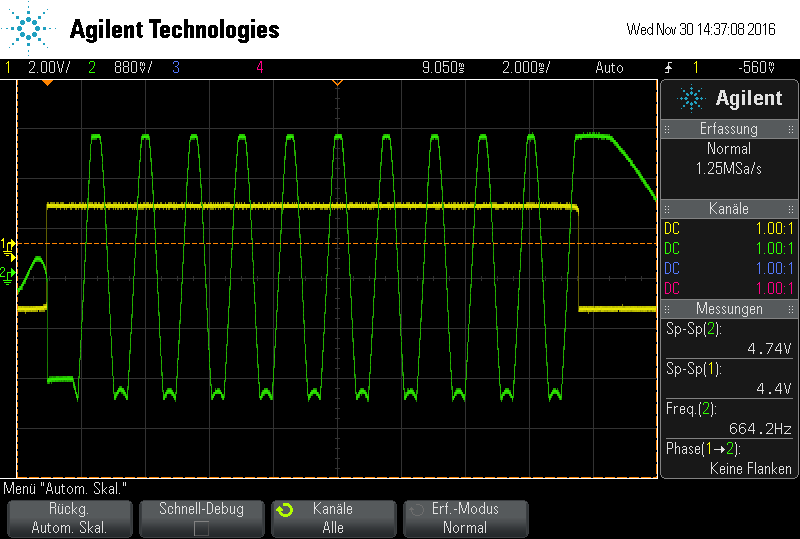
\includegraphics[width=10cm]{images/schwingung.png}
	\captionof{figure}{Thermodruck der ungedämpften Schwingung nach Anregung durch Rechteckschwingung}
	\label{fig:thermoexpon_ung}
\end{center}
Zur Bestimmung der Abklingdauer der gedämpften Schwingung, welche in Abbildung \ref{fig:thermoexpon} dargestellt ist, werden mithilfe eines Peak-Detection-Algorithmus die Maxima bestimmt und mit diesen mit einem Exponentialansatz $U_{\text{max}}(t)=U_0\exp\left(-t/\tau\right) $ eine Ausgleichsrechnung durchgeführt. In Abbildung \ref{fig:expfit} sind der nicht-lineare Fit sowie die Messwerte dargestellt. Die Positionen der Peaks sind in Tabelle \ref{tab:peak} aufgeführt.\\
Aus der nicht-linearen Ausgleichsrechnung ergibt sich die Abklingdauer von
\begin{align*}
\tau_{exp}=\SI{4.1(2)}{\milli\second}\,.
\end{align*}
\newpage
\begin{center}
	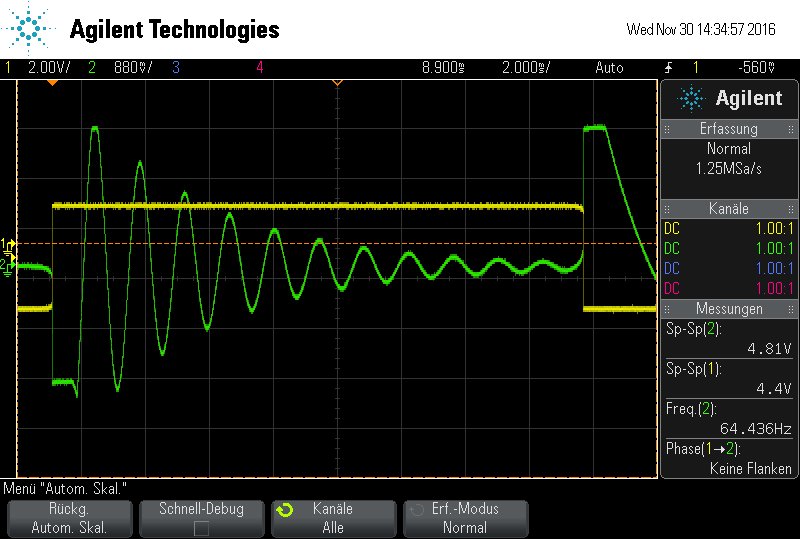
\includegraphics[width=10cm]{images/schwinggen.png}
	\captionof{figure}{Thermodruck des exponentiellen Abfalls nach Anregung durch Rechteckschwingung}
	\label{fig:thermoexpon}
\end{center}
\begin{center}
	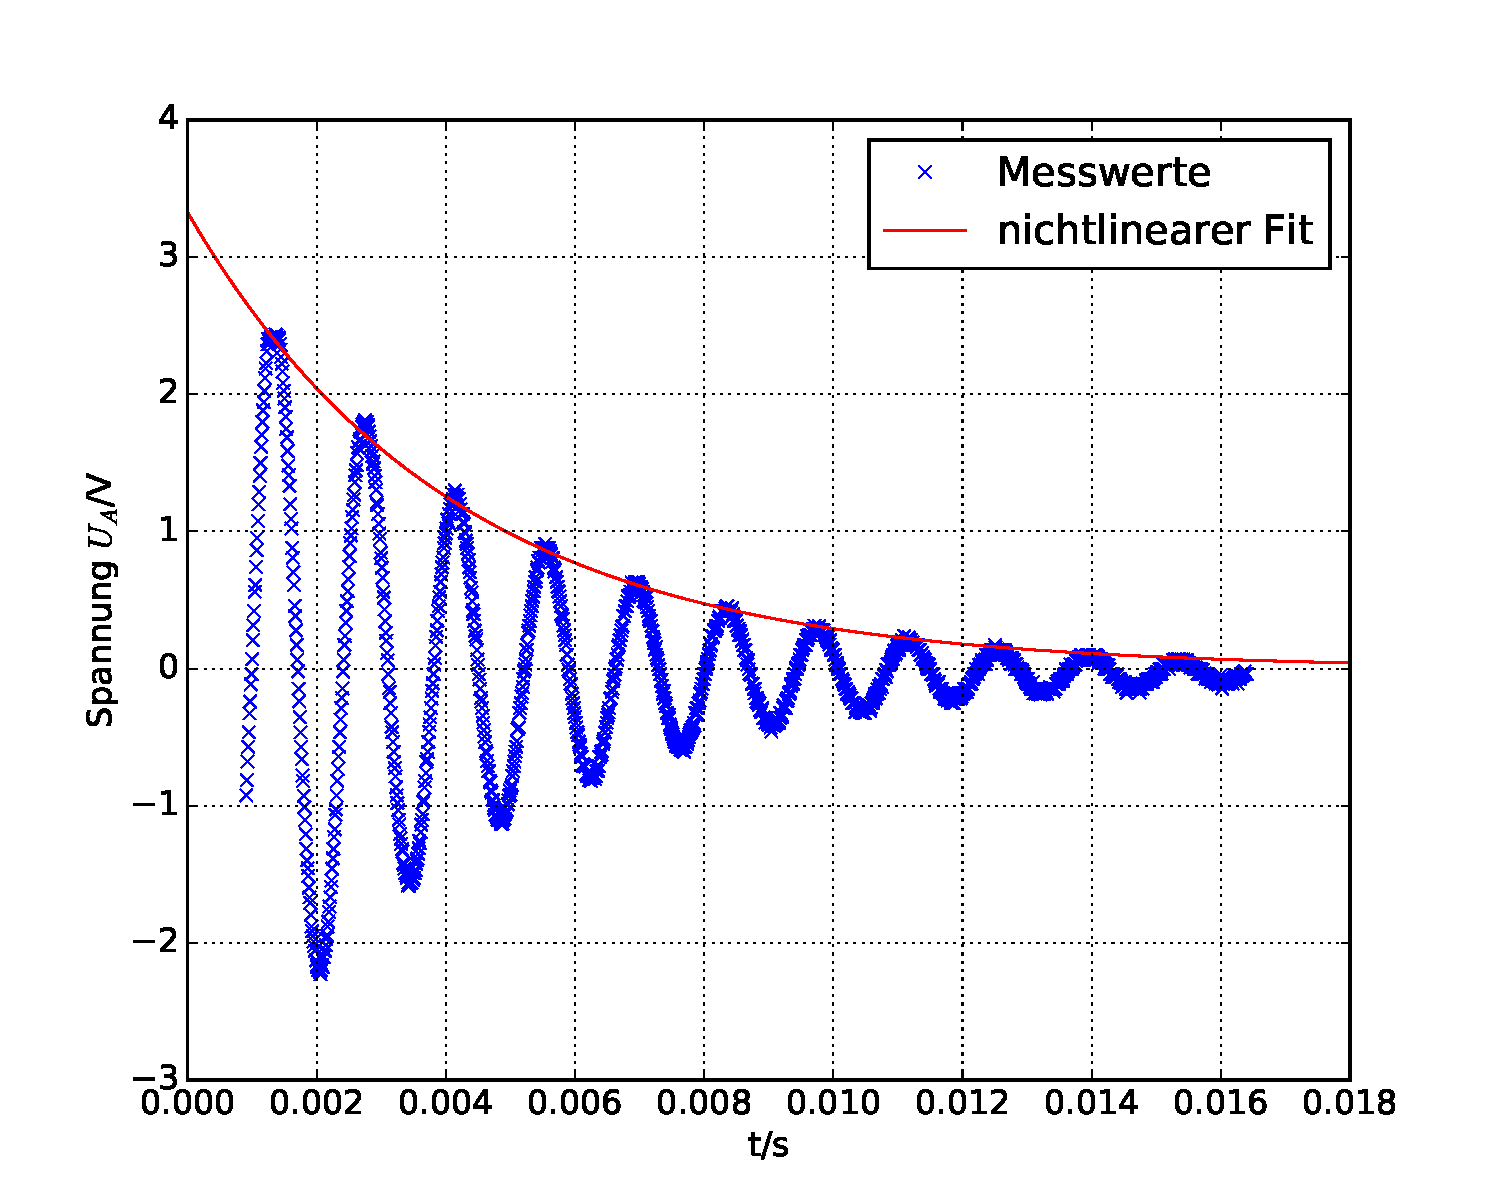
\includegraphics[width=10cm]{images/schwing_abfall.pdf}
	\captionof{figure}{Messwerte zum Schwingabfall des Signals und nichtlinearer Fit der Maxima}
	\label{fig:expfit}
\end{center}

\section{Diskussion}

\subsection{Frequenzgang und Phasengang des gegengekoppelten Verstärkers}
Die experimentell bestimmten Verstärkungen liegen nur im Falle von $R_n=\SI{1}{\kilo\ohm}$ und bei $R_n=\SI{570}{\ohm}$ mit 0.02\% und 70\% Abweichung vom Theoriewert in der gleichen Grö"senordnung wie der Theoriewert. \\
Desweiteren ergeben sich bei $R_n=\SI{100}{\ohm}$ und bei $R_n=\SI{570}{\ohm}$ physikalisch nicht sinnvolle negative Leerlaufverstärkungen. Das eigentlich konstante Verstärkungs-Bandbreite-Produkt ist hier auch für jeden Widerstand unterschiedlich, was jedoch aus den vorherigen Abweichungen resultiert. \\
Desweiteren ist auffällig, dass die Fehler der ermittelten Grenzfrequenzen sehr hoch sind. Dies resultiert aus dem Anwenden der Exponentialfunktion auf die ermittelten Fit-Parameter, deren Fehler noch nicht diese Grö"se hatte. \\
Der Theoriewert der Steigung ist m=-1 (für einen Tiefpass), die Steigungen der verschiedenen Konfigurationen schwanken zwischen -0.897 und -0.819, haben also signifikante Abweichungen vom theoretisch erwarteten Wert. \\
Bezüglich des Phasenganges ist in der Abbildung deutlich zu erkennen, dass der Absolutbetrag der Phasendifferenz zwischen Eingangs- und Ausgangsspannung mit steigender Frequenz abnimmt. Dies ist konsistent mit Gleichung \ref{eq:tiefpass_phase}, wonach zwischen Phase $\phi$ und Frequenz $f=2\pi\omega$ die Beziehung 
\begin{align*}
\phi=\arctan\left(-\frac{f}{f_g}\right)
\end{align*}
gilt. Durch die Punktsymmetrie des $\arctan$ ergibt sich so ein dem aufgenommenen Bild ähnlicher Verlauf.

\subsection{Der Umkehrintegrator und -differentiator}
Der Umkehrintegrator funktioniert wie erwartet, wie an den aufgenommen Bilder der Oszilloskopausgabe zu sehen ist. Da für den Integrator die Beziehung $U_A\propto\omega^{-1}$ gelten soll, lautet der Theoriewert $m=-1$. Die lineare Regression ergab einen Wert von  \\$m=-0.754\pm0.040$, welcher um 24.6\% vom Theoriewert abweicht. \\
Der Umkehrdifferentiator arbeitete, wie auf den aufgenommenen Bildern zu sehen ist, wie erwartet. Jedoch ergab sich eine starke Abweichung von der Beziehung $U_A\propto\omega$. Der theoretisch erwartete Wert für die Steigung m war m=1, jedoch ergab die lineare Regression einen Wert von $m = -0.797 \pm 0.039$. Dies lässt sich auf einen systematischen Fehler im Aufbau oder in Apparatur zurückführen.

\subsection{Der Schmitt-Trigger}
Der Schmitt-Trigger arbeitet nicht vollständig wie erwartet, die Kippspannung weicht mit 127\% signifikant vom theoretisch erwarteten Wert ab. Zudem ist beim Signalverlauf zu erkennen, dass keine perfekte Rechteckspannung erzeugt wurde, sondern signifikant die Form noch vom eingehenden Sinus-Signal beeinflusst wurde. Hier ist von einem systematischen Fehler im Aufbau oder der Apparatur auszugehen.

\subsection{Der Dreiecksgenerator}
Der Dreiecksgenerator liefert wie erwartet ein Dreieckssignal. Die experimentell \\bestimmte Frequenz des Dreieckgenerators weicht um 10.70\% vom berechneten Theoriewert ab. Jedoch ist eine Asymmetrie der der Extremwerte festzustellen, was auch an der Abflachung des Signals zu erkennen ist. Hier kann von einem systematischen Fehler, wie z.B. der falschen Parameterwahl, ausgegangen werden.

\subsection{Die Schwingungsdifferentialschaltung}
Die Schwingungsdifferentialschaltung funktioniert, wie auf den Thermodrucken zu sehen ist, wie erwartet. Für die Frequenz der Schaltung ergibt ein experimentell bestimmter Wert von $f_{exp}=\SI{664.2}{\hertz}$, was mit 8.2\% vom Theoriewert $f_{theo}=\SI{723.43}{\hertz}$ abweicht. \\
Die Abklingdauer liegt bei $\tau_{exp}=\SI{4.1(2)}{\milli\second}$, diese weicht um 8,9\% vom Theoriewert ab, dies liegt au"serhalb des angegebenen statistischen Fehlers.

\section{Quellen}
{[1]} Physikalisches Praktikum, TU Dortmund: \\
\textit{Versuchsanleitung zu Versuch 51: Schaltungen mit Operationsverstärkern}\\
http://129.217.
224.2/HOMEPAGE/PHYSIKER/MASTER/SKRIPT/V51.pdf (letzte Version vom 02.01.2017, 11:10)\\

\section{Anhang}

\begin{table}[H]
	\centering
	\captionof{table}{Frequenzgang des gegengekoppelten Verstärkers für $R_n=\SI{1}{\kilo\ohm}$}
	\label{tab:ggverst_a}
	\hskip-1.50cm
	\begin{tabular}{r r r}
		\toprule
		$f / \si{\kilo\hertz}$ & $U_A/\si{\volt}$ & $U_E/\si{\volt}$ \\
		\midrule
		0.10	&	2.57	&	2.61 \\
		0.25	&	2.57	&	2.65 \\
		0.50	&	2.57	&	2.61 \\
		0.50	&	2.61	&	2.69 \\
		1.00	&	2.61	&	2.69 \\
		5.00	&	2.57	&	2.65 \\
		10.00	&	2.92	&	3.02 \\
		15.00	&	3.38	&	3.42 \\
		20.00	&	2.05	&	2.09 \\
		50.00	&	1.51	&	1.57 \\
		75.00	&	1.57	&	1.65 \\
		100.00	&	1.59	&	1.69 \\
		200.00	&	1.53	&	1.77 \\
		300.00	&	1.43	&	1.87 \\
		500.00	&	1.39	&	2.13 \\
		1000.00	&	0.98	&	2.25 \\
		2000.00	&	0.56	&	2.37 \\
		5000.00	&	0.19	&	2.33 \\
		10000.00	&	0.09	&	2.14 \\
		\bottomrule
	\end{tabular}
\end{table}

\begin{table}[H]
	\centering
	\captionof{table}{Frequenzgang des gegengekoppelten Verstärkers für $R_n=\SI{100}{\ohm}$}
	\label{tab:ggverst_b}
	\hskip-1.50cm
	\begin{tabular}{r r r}
		\toprule
		$f / \si{\kilo\hertz}$ & $U_A/\si{\volt}$ & $U_E/\si{\volt}$ \\
		\midrule
		0.10	&	2.61	&	2.69 \\
		0.25	&	2.57	&	2.69 \\
		0.50	&	2.57	&	2.61 \\
		0.50	&	2.61	&	2.65 \\
		1.00	&	2.61	&	2.69 \\
		5.00	&	2.53	&	2.61 \\
		10.00	&	2.97	&	2.97 \\
		15.00	&	3.38	&	3.42 \\
		20.00	&	2.01	&	2.05 \\
		50.00	&	1.57	&	1.61 \\
		75.00	&	1.63	&	1.67 \\
		100.00	&	1.53	&	1.63 \\
		200.00	&	1.53	&	1.71 \\
		300.00	&	1.57	&	1.83 \\
		500.00	&	1.71	&	2.11 \\
		1000.00	&	1.45	&	2.25 \\
		2000.00	&	0.88	&	2.21 \\
		5000.00	&	0.33	&	2.17 \\
		10000.00	&	0.17	&	1.97 \\
		\bottomrule
	\end{tabular}
\end{table}

\begin{table}[H]
	\centering
	\captionof{table}{Frequenzgang des gegengekoppelten Verstärkers für $R_n=\SI{570}{\ohm}$}
	\label{tab:ggverst_c}
	\hskip-1.50cm
	\begin{tabular}{r r r}
		\toprule
		$f / \si{\kilo\hertz}$ & $U_A/\si{\volt}$ & $U_E/\si{\volt}$ \\
		\midrule
		0.10	&	2.57	&	2.61 \\
		0.25	&	2.61	&	2.73 \\
		0.50	&	2.57	&	2.65 \\
		0.50	&	2.57	&	2.65 \\
		1.00	&	2.57	&	2.65 \\
		5.00	&	2.57	&	2.69 \\
		10.00	&	2.97	&	2.97 \\
		15.00	&	3.38	&	3.42 \\
		20.00	&	2.09	&	2.09 \\
		50.00	&	1.55	&	1.61 \\
		75.00	&	1.57	&	1.63 \\
		100.00	&	1.53	&	1.69 \\
		200.00	&	1.49	&	1.73 \\
		300.00	&	1.55	&	1.83 \\
		500.00	&	1.61	&	2.13 \\
		1000.00	&	1.21	&	2.25 \\
		2000.00	&	0.72	&	2.25 \\
		5000.00	&	0.26	&	2.25 \\
		10000.00	&	0.12	&	2.06 \\
		\bottomrule
	\end{tabular}
\end{table}

\begin{table}[H]
	\centering
	\captionof{table}{Frequenzgang des gegengekoppelten Verstärkers für $R_n=\SI{100}{\kilo\ohm}$}
	\label{tab:ggverst_d}
	\hskip-1.50cm
	\begin{tabular}{r r r}
		\toprule
		$f / \si{\kilo\hertz}$ & $U_A/\si{\volt}$ & $U_E/\si{\volt}$ \\
		\midrule
		0.10	&	2.33	&	2.65 \\
		0.25	&	2.37	&	2.69 \\
		0.50	&	2.33	&	2.61 \\
		0.50	&	2.33	&	2.61 \\
		1.00	&	2.37	&	2.69 \\
		5.00	&	2.13	&	3.10 \\
		10.00	&	2.17	&	3.78 \\
		15.00	&	2.09	&	4.38 \\
		20.00	&	1.25	&	3.18 \\
		50.00	&	0.50	&	2.81 \\
		75.00	&	0.32	&	2.25 \\
		100.00	&	0.19	&	2.05 \\
		200.00	&	0.14	&	1.81 \\
		300.00	&	0.12	&	1.75 \\
		500.00	&	0.10	&	2.09 \\
		1000.00	&	0.04	&	2.37 \\
		2000.00	&	0.02	&	2.41 \\	
		\bottomrule
	\end{tabular}
\end{table}
		

\begin{table}[H]
	\centering
	\captionof{table}{Phasenverschiebung $\phi$ in Abhängigkeit von der Frequenz $f$}
	\label{tab:phase}
	\hskip-1.50cm
	\begin{tabular}{r r}
		\toprule
		$f / \si{\hertz}$ & $\phi / ^{\circ}$ \\
		\midrule
		20	&	172	\\
		30	&	173	\\
		40	&	173	\\
		50	&	173	\\
		100	&	172	\\
		200	&	172	\\
		500	&	171	\\
		1000	&	172	\\
		10000	&	174	\\
		20000	&	176	\\
		30000	&	179	\\
		40000	&	189	\\
		50000	&	200	\\
		60000	&	214	\\
		70000	&	224	\\
		80000	&	234	\\
		90000	&	240	\\
		100000	&	247	\\
		150000	&	264	\\
		200000	&	272	\\
		250000	&	284	\\
		300000	&	288	\\
		350000	&	292	\\
		400000	&	298	\\
		500000	&	305	\\
		600000	&	314	\\
		700000	&	322	\\
		800000	&	334	\\
		900000	&	340	\\
		1000000	&	350	\\
		1200000	&	360	\\
		1500000	&	337	\\
		\bottomrule
	\end{tabular}
\end{table}

\begin{table}[H]
	\centering
	\captionof{table}{Werte der Ausgangsspannung des Umkehrintegrators in Abhängigkeit von $f$}
	\label{tab:integrator}
	\hskip-1.50cm
	\begin{tabular}{r r}
		\toprule
		$f / \si{\kilo\hertz}$ & $U_A / \si{\volt}$ \\
		\midrule
		10000 & 0.19 \\
		7500  & 0.27 \\
		5000  & 0.38 \\
		2500  & 0.76 \\
		1000  & 1.49 \\
		900   & 1.57 \\
		800   & 1.65 \\
		700   & 1.73 \\
		600   & 1.81 \\
		500   & 1.87 \\
		400   & 2.01 \\
		300   & 1.75 \\
		200   & 1.69 \\
		100   & 2.41 \\
		50    & 2.41 \\
		\bottomrule
	\end{tabular}
\end{table}

\begin{table}[H]
	\centering
	\captionof{table}{Werte der Ausgangsspannung des Umkehrdifferentiators in Abhängigkeit von $f$}
	\label{tab:differentiator}
	\hskip-1.50cm
	\begin{tabular}{r r}
		\toprule
		$f / \si{\kilo\hertz}$ & $U_A / \si{\volt}$ \\
		\midrule
		10000 & 0.18 \\
		7500  & 0.27 \\
		5000  & 0.40 \\
		2500  & 0.77 \\
		1000  & 1.45 \\
		900   & 1.53 \\
		800   & 1.59 \\
		700   & 1.67 \\
		600   & 1.73 \\
		500   & 1.79 \\
		400   & 1.75 \\
		300   & 1.61 \\
		200   & 1.55 \\
		100   & 1.51 \\
		50    & 1.49 \\
		\bottomrule
	\end{tabular}
\end{table}

\begin{table}[H]
	\centering
	\captionof{table}{Peaks der gedämpften Schwingung}
	\label{tab:peak}
	\hskip-1.50cm
	\begin{tabular}{r r}
		\toprule
		$t/\si{\milli\second}$ & $U_A / \si{\volt}$ \\
		\midrule
		1.36 & 2.44 \\
		2.75 & 1.81 \\
		2.91 & 1.36 \\
		4.14 & 1.30 \\
		5.54 & 0.910 \\
		6.93 & 0.631 \\
		8.35 & 0.455 \\
		9.71 & 0.313 \\
		9.91 & 0.227 \\
		11.1 & 0.238 \\
		12.5 & 0.172 \\
		13.9 & 0.101 \\
		15.3 & 0.065 \\
		\bottomrule
	\end{tabular}
\end{table}


\end{document}
